\chapter{Divide-and-Conquer}

\section{The maximum-subarray problem}

\begin{enumerate}

\item[4.1{-}1]{What does \textsc{Find-Maximum-Subarray} return when all
elements of A are negative?}

\begin{framed}
A subarray with only the largest negative element of $A$.
\end{framed}

\item[4.1{-}2]{Write pseudocode for the brute-force method of solving the
maximum-subarray problem. Your procedure should run in $\Theta(n^2)$ time.}

\begin{framed}
The pseudocode is stated below.\\
\begin{algorithm}[H]
\SetAlgoNoEnd\DontPrintSemicolon
\BlankLine
\SetKwFunction{algo}{FindMaximumSubarray-BruteForce}
\SetKwProg{myalg}{}{}{}
\myalg{\algo{A}}{%
\nl $low = 0$\;
\nl $high = 0$\;
\nl $sum = -\infty$\;
\nl \For{$i = 1$ \KwTo $A.length$}{%
\nl   $cursum = 0$\;
\nl   \For {$j = i$ \KwTo $A.length$}{%
\nl     $cursum = cursum + A[j]$\;
\nl     \If{$cursum > sum$}{%
\nl       $sum = cursum$\;
\nl       $low = i$\;
\nl       $high = j$\; } } }
\nl \Return{$low, high, sum$} }
\end{algorithm}
\end{framed}

\item[4.1{-}3]{Implement both the brute-force and recursive algorithms for the
maximum-subarray problem on your own computer. What problem size $n_0$ gives
the crossover point at which the recursive algorithm beats the brute-force
algorithm? Then, change the base case of the recursive algorithm to use the
brute-force algorithm whenever the problem size is less than $n_0$. Does
that change the crossover point?}



\begin{framed}
Figure below in the lhs ilustrates the crossover point between the
BruteForce and Recursive solutions in my machine. In that comparison, $n_0
\approx 52$. Figure below in the rhs ilustrates the crossover point
between the BruteForce and Mixed solutions in my machine. The crossover point
does not change but the Mixed solution becomes as fast as the BruteForce
solution when the problem size is lower than 52.

\begin{center}
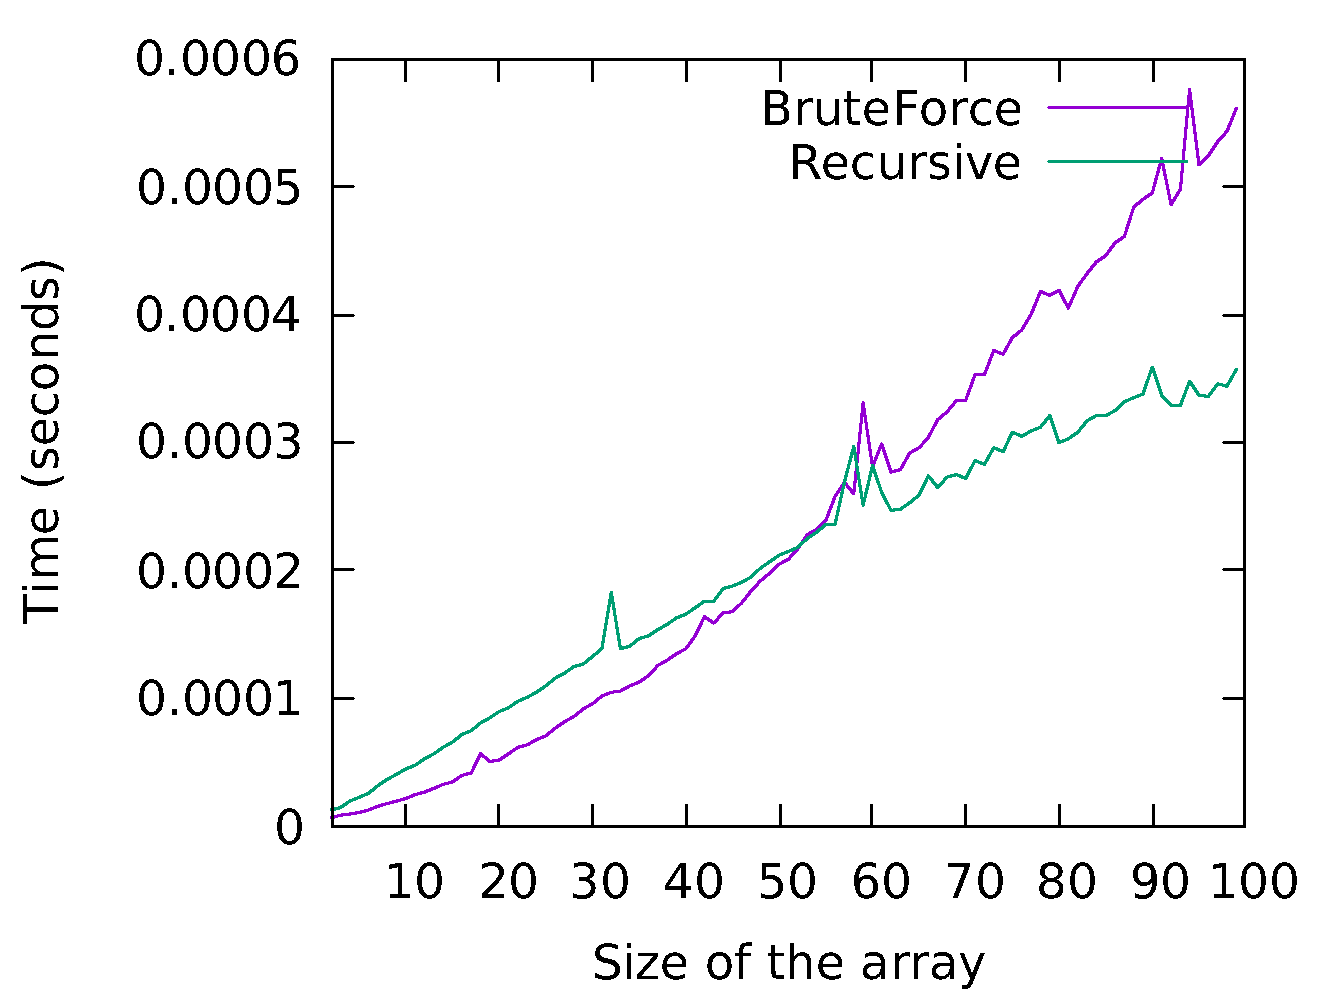
\includegraphics[width=0.35\textwidth]{images/4_1_3_1.pdf}
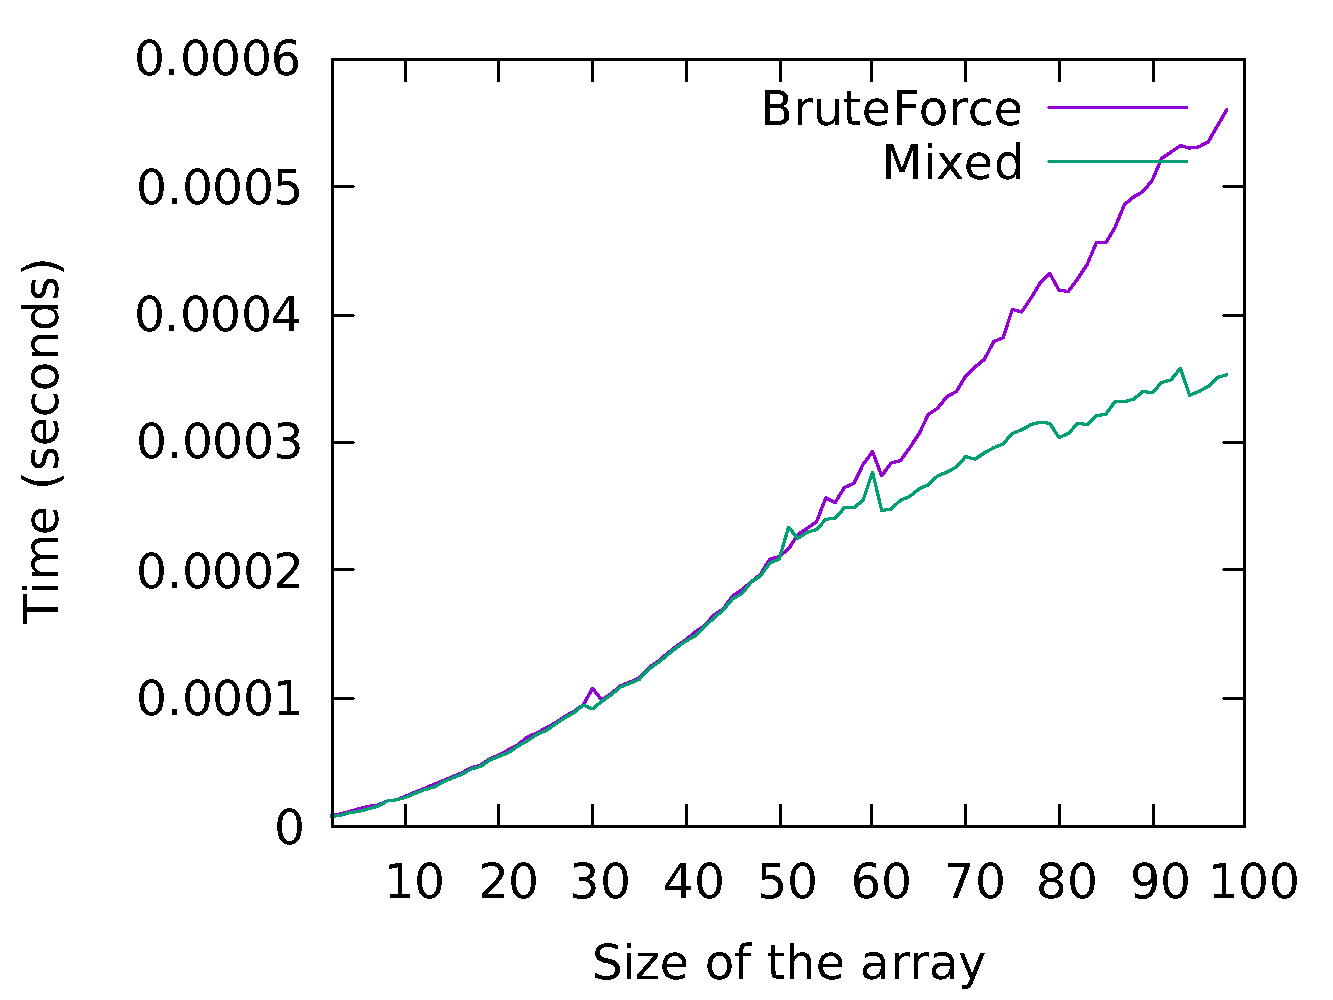
\includegraphics[width=0.35\textwidth]{images/4_1_3_2.pdf}
\end{center}
\end{framed}

\item[4.1{-}4]{Suppose we change the definition of the maximum-subarray problem
to allow the result to be an empty subarray, where the sum of the values of an
empty subarray is 0. How would you change any of the algorithms that do not
allow empty subarrays to permit an empty subarray to be the result?}

\begin{framed}
The BruteForce algorithm (stated above in Question 4.1{-}2) can be updated just
by modifying line 3 to $sum = 0$, instead of $sum = -\infty$. In that case, if
there is no subarray whose sum is greater than zero, the algorithm will return
a invalid subarray ($low = 0, high = 0, sum = 0$), which will denote the empty
subarray.

The Recursive algorithm (stated in Section 4.1) can be updated as follows. In
the \textsc{Find-Max-Crossing-Subarray} routine, update lines 1 and 8 to
initialize $left \mhyphen sum$ and $right \mhyphen sum$ to 0, instead of
$-\infty$. Also initialize $max \mhyphen left$ (after line 1) and $max \mhyphen
right$ (after line 8) to 0. In the \textsc{Find-Maximum-Subarray} routine,
surround the return statement of line 2  with a conditional that
verifies if $A[low]$ is greater than zero. If it is, return the values as it was
before. If it is not, return a invalid subarray (denoted by $low = 0$ and
$high = 0$) and the sum as zero.
\end{framed}

\item[4.1{-}5]{Use the following ideas to develop a nonrecursive, linear-time
algorithm for the maximum-subarray problem. Start at the left end of the
array, and progress toward the right, keeping track of the maximum subarray
seen so far. Knowing a maximum subarray of $A[1, \dots, j]$, extend the answer
to find a maximum subarray ending at index $j + 1$ by using the following
observation: a maximum subarray of $A[1, \dots, j + 1]$ is either a maximum
subarray of $A[1, \dots, j]$ or a subarray $A[i, \dots, j + 1]$, for some
$1 \le i \le j + 1$. Determine a maximum subarray of the form $A[i, \dots,
j + 1]$ in constant time based on knowing a maximum subarray ending at index
$j$.}

\begin{framed}
The pseudocode is stated below.\\
\begin{algorithm}[H]
\SetAlgoNoEnd\DontPrintSemicolon
\BlankLine
\SetKwFunction{algo}{FindMaximumSubarray-Linear}
\SetKwProg{myalg}{}{}{}
\myalg{\algo{A}}{%
\nl $low = 0$\;
\nl $high = 0$\;
\nl $sum = 0$\;
\nl $current \mhyphen low = 0$\;
\nl $current \mhyphen sum = 0$\;
\nl \For{$i = 1$ \KwTo $A.length$}{%
\nl   $current \mhyphen sum = \max(A[i], current \mhyphen sum + A[i])$\;
\nl   \If{$current \mhyphen sum == A[i]$}{%
\nl     $current \mhyphen low = i$\; }
\nl   \If{$current \mhyphen sum > sum$}{%
\nl     $low = current \mhyphen low$\;
\nl     $high = i$\;
\nl     $sum = current \mhyphen sum$\; } }
\nl \Return{$low, high, sum$} }
\end{algorithm}

\vspace{0.5mm}

We can make it a little faster (twice as fast on my machine) by avoiding
executing lines 7, 8, and 10 when not necessary.\\
\begin{algorithm}[H]
\SetAlgoNoEnd\DontPrintSemicolon
\BlankLine
\SetKwFunction{algo}{FindMaximumSubarray-Linear-Optimized}
\SetKwProg{myalg}{}{}{}
\myalg{\algo{A}}{%
\nl $low = 0$\;
\nl $high = 0$\;
\nl $sum = 0$\;
\nl $current \mhyphen low = 0$\;
\nl $current \mhyphen sum = 0$\;
\nl \For{$i = 1$ \KwTo $A.length$}{%
\nl   \If{$current \mhyphen sum + A[i] \le 0$}{%
\nl     $current \mhyphen sum = 0$\; }
\nl   \Else{%
\nl     $current \mhyphen sum = current \mhyphen sum + A[i]$\;
\nl     \If{$current \mhyphen sum == A[i]$}{%
\nl       $current \mhyphen low = i$\; }
\nl     \If{$current \mhyphen sum > sum$}{%
\nl       $low = current \mhyphen low$\;
\nl       $high = i$\;
\nl       $sum = current \mhyphen sum$\; } } }
\nl \Return{$low, high, sum$} }
\end{algorithm}
\end{framed}

\end{enumerate}

\newpage

\section{Strassen's algorithm for matrix multiplication}

\begin{enumerate}

\item[4.2{-}1]{Use Strassen's algorithm to compute the matrix product
\[
\begin{bmatrix}
  1 & 3\\
  7 & 5
\end{bmatrix}
\begin{bmatrix}
  6 & 8\\
  4 & 2
\end{bmatrix}
.
\]
Show your work.
}

\begin{framed}
Let
\[
  A = \begin{bmatrix} 1 & 3\\ 7 & 5 \end{bmatrix},
  B = \begin{bmatrix} 6 & 8\\ 4 & 2 \end{bmatrix},
\]
and $C = A \cdot B$. To compute $C$ using Strassen's algorithm, we start by
computing the $S_i$ matrices:
\begin{equation*}
\begin{aligned}
S_1 \; &= \; B_{12} - B_{22} \; = \; 8 - 2 \; = \; 6,\\
S_2 \; &= \; A_{11} + A_{12} \; = \; 1 + 3 \; = \; 4,\\
S_3 \; &= \; A_{21} + A_{22} \; = \; 7 + 5 \; = \; 12,\\
S_4 \; &= \; B_{21} - B_{11} \; = \; 4 - 6 \; = \; -2,\\
S_5 \; &= \; A_{11} + A_{22} \; = \; 1 + 5 \; = \; 6,\\
S_6 \; &= \; B_{11} + B_{22} \; = \; 6 + 2 \; = \; 8,\\
S_7 \; &= \; A_{12} + A_{22} \; = \; 3 - 5 \; = \; -2,\\
S_8 \; &= \; B_{21} + B_{22} \; = \; 4 + 2 \; = \; 6,\\
S_9 \; &= \; A_{11} - A_{21} \; = \; 1 - 7 \; = \; -6,\\
S_{10} \; &= \; B_{11} + B_{12} \; = \; 6 + 8 \; = \; 14.
\end{aligned}
\end{equation*}

Then we compute the $P_i$ matrices:
\begin{equation*}
\begin{aligned}
  P_1 \; &= \; A_11 \cdot S_1 \; &&= \; 1 \cdot 6 \; &&= \; 6,\\
  P_2 \; &= \; S_2 \cdot B_22 \; &&= \; 4 \cdot 2 \; &&= \; 8,\\
  P_3 \; &= \; S_3 \cdot B_11 \; &&= \; 12 \cdot 6 \; &&= \; 72,\\
  P_4 \; &= \; A_22 \cdot S_4 \; &&= \; 5 \cdot (-2) \; &&= \; -10,\\
  P_5 \; &= \; S_5 \cdot S_6 \; &&= \; 6 \cdot 8 \; &&= \; 48,\\
  P_6 \; &= \; S_7 \cdot S_8 \; &&= \; (-2) \cdot 6 \; &&= \; -12,\\
  P_7 \; &= \; S_9 \cdot S_10 \; &&= \; (-6) \cdot 14 \; &&= \; -84.
\end{aligned}
\end{equation*}

Using matrices $S_i$ and $P_i$, we compute $C$:
\[
C =
\begin{bmatrix}
(P_5 + P_4 - P_2 + P_6) & (P_2 + P_2)\\ (P_3 + P_4) & (P_5 + P_1 - P_3 - P_7)
\end{bmatrix}
=
\begin{bmatrix}
18 & 14\\ 62 & 66
\end{bmatrix}
.
\]
\end{framed}

\newpage

\item[4.2{-}2]{Write pseudocode for Strassen's algorithm.}

\begin{framed}
The pseudocode is stated below.\\
\begin{algorithm}[H]
\SetAlgoNoEnd\DontPrintSemicolon
\BlankLine
\SetKwFunction{algo}{Square-Matrix-Multiply-Strassen}
\SetKwProg{myalg}{}{}{}
\myalg{\algo{A, B}}{%
\nl $n = A.rows$\;
\nl let $C$ be a new $n \times n$ matrix\;
\nl \If{$n == 1$}{%
\nl   $c_{11} = a_{11} \cdot b_{11}$\; }
\nl \Else{%
\nl   partition $A, B$, and $C$ as into $n/2 \times n/2$ submatrices\;
\nl   let $S_1, S_2, \dots, S_{10}$ be new $n/2 \times n/2$ matrices\;
\nl   let $P_1, P_2, \dots, P_7$ be new $n/2 \times n/2$ matrices\;
\nl   $S_1 = B_{12} - B_{22}$\;
\nl   $S_2 = A_{11} + A_{12}$\;
\nl   $S_3 = A_{21} + A_{22}$\;
\nl   $S_4 = B_{21} - B_{11}$\;
\nl   $S_5 = A_{11} + A_{22}$\;
\nl   $S_6 = B_{11} + B_{22}$\;
\nl   $S_7 = A_{12} - A_{22}$\;
\nl   $S_8 = B_{21} + B_{22}$\;
\nl   $S_9 = A_{11} - A_{21}$\;
\nl   $S_{10} = B_{11} - B_{12}$\;
\nl   $P_1 =$ \texttt{Square-Matrix-Multiply-Strassen}($A_{11}, S_1$)\;
\nl   $P_2 =$ \texttt{Square-Matrix-Multiply-Strassen}($S_2, B_{22}$)\;
\nl   $P_3 =$ \texttt{Square-Matrix-Multiply-Strassen}($S_3, B_{11}$)\;
\nl   $P_4 =$ \texttt{Square-Matrix-Multiply-Strassen}($A_{22}, S_4$)\;
\nl   $P_5 =$ \texttt{Square-Matrix-Multiply-Strassen}($S_5, S_6$)\;
\nl   $P_6 =$ \texttt{Square-Matrix-Multiply-Strassen}($S_7, S_8$)\;
\nl   $P_7 =$ \texttt{Square-Matrix-Multiply-Strassen}($S_9, S_{10}$)\;
\nl   $C_{11} = P_5 + P_4 - P_2 + P_6$ \;
\nl   $C_{12} = P_1 + P_2$ \;
\nl   $C_{21} = P_3 + P_4$ \;
\nl   $C_{22} = P_5 + P_1 - P_3 - P_7$ \; }
\nl \Return{$C$} }
\end{algorithm}
\end{framed}

\item[4.2{-}3]{How would you modify Strassen's algorithm to multiply $n \times
n$ matrices in which $n$ is not an exact power of 2? Show that the resulting
algorithm runs in time $\Theta(n^{\lg 7})$.}

\begin{framed}
Pad each input $n \times n$ matrix (rows and columns) with $m - n$ zeros,
resulting in an $m \times m$ matrix, where $m = 2^{\ceil{\lg n}}$. After
computing the final matrix, cut down the last $m - n$ rows and $m - n$ columns
(which will be zeros).

Padding the matrix with zeros is done once, in the root of the recursion tree,
and takes $O(m^2)$. Since we now have an $m \times m$ matrix, the algorithm runs
in $\Theta(m^{\lg 7}) + O(m^2) = \Theta(m^{\lg 7})$. We have that
$n \le m <  2^{(\lg n) + 1} = 2^{\lg n} \cdot 2 = 2n.$ Thus, the
algorithm runs in $\Theta((2n)^{\lg 7}) = \Theta(n^{\lg 7})$.
\end{framed}

\item[4.2{-}4]{What is the largest $k$ such that if you can multiply
$3 \times 3$ matrices using $k$ multiplications (not assuming commutativity of
multiplication), then you can multiply $n \times n$ matrices in time
$o(n^{\lg 7})$?  What would the running time of this algorithm be?
}

\begin{framed}
If we modify the \textsc{Square-Matrix-Multiply-Recursive} algorithm to
partition the matrices into $n/3 \times n/3$ submatrices, we would have the
following recurrence:
\[
T(n) = \Theta(1) + 27 T(n/3) + \Theta(n^2) = 27 T(n/3) + \Theta(n^2).
\]

Let's proceed to understand a little more about the above recurrence. Let $A$
and $B$ be the two input matrices in each node of the above recursion tree.
Like in the original \textsc{Square-Matrix-Multiply-Recursive} algorithm, our
modified version will take $\Theta(1)$ to partition $A$ and $B$ into $n/3 \times
n/3$ submatrices. In each node of the tree, the product of $A$ and $B$ is
recursively computed by the products of their submatrices. Since the number of
recursive (submatrices) products to compute $A \cdot B$ in each node of the
recurstion tree is 27 and each of these submatrices is $3$ times smaller than
$A$ and $B$, the 27 recursive products takes $27 T(n/3)$. Finally, the number of
summations to compute the final matrix is
$\Theta(3 \cdot 9 \cdot n^2/3) = \Theta(n^2)$.

If after partitioning $A$ and $B$ into $n/3 \times n/3$ submatrices we can
compute their product with $k$ multiplications (instead of 27), we would have
the following recurrence:
\[
T(n) = \Theta(1) + k T(n/3) + \Theta(n^2) = k T(n/3) + \Theta(n^2),
\]

We can solve the above recurrence using the master method. We have
$f(n) = n^2$ and $n^{log_b a} = n^{\log_3 k}$. Using the first case of the master
method, we have
\[
\Forall k \; | \log_3 k > 2, \; n^2 = O(n^{(\log_3 k) - \epsilon}), \; 0 \le \epsilon \le \log_3 k - 2,
\]
which implies
\[
T(n) = \Theta(n^{\log_3 k}).
\]

Since $\log_3 21 < \lg 7 < \log_3 22$, the largest value for $k$ is 21. Its
running time would be $n^{\log_3 21} \approx n^{2.7712}$.

\end{framed}

\item[4.2{-}5]{V. Pan has discovered a way of multiplying $68 \times 68$
matrices using 132,464 multiplications, a way of multiplying $70 \times 70$
matrices using 143,640 multiplications, and a way of multiplying $72 \times 72$
matrices using 155,424 multiplications. Which method yields the best asymptotic
running time when used in a divide-and-conquer matrix-multiplication algorithm?
How does it compare to Strassen's algorithm?}

\begin{framed}
The algorithms would take:
\begin{itemize}
  \item $n^{\log_{68} 132,464} \approx n^{2.795128}$,
  \item $n^{\log_{70} 143,640} \approx n^{2.795122}$,
  \item $n^{\log_{72} 155,424} \approx n^{2.795147}$.
\end{itemize}

The fastest is the one that multiplies $70 \times 70$ matrices, but all of them
are faster then the Strassen's algorithm.
\end{framed}

\item[4.2{-}6]{How quickly can you multiply a $k n \times n$ matrix by an
$n \times k n$ matrix, using Strassen's algorithm as a subroutine? Answer the
same question with the order of the input matrices reversed.}

\begin{framed}
Let $A$ and $B$ be $kn \times n$ and $n \times k n$ matrices, respectivelly. We
can compute $A \cdot B$ as follows:
\begin{enumerate}
\item Partition $A$ and $B$ into $k$ submatrices $A_1, \dots, A_k$ and $B_1,
\dots, B_k$, each one of size $n \times n$.
\item Compute the desired submatrices $C_{ij}$ of the result matrix $C$ by the
product of $A_i \cdot B_j$. Use the Strassen's algorithm to compute each of
those products.
\end{enumerate}

Since each of the $k^2$ products takes $\Theta(n^{\lg 7})$, this algorithm
runs in $\Theta(k^2 n^{\lg 7})$.

We can compute $B \cdot A$ as follows:
\begin{enumerate}
\item Partition $A$ and $B$ into $k$ submatrices $A_1, \dots, A_k$ and $B_1,
\dots, B_k$, each one of size $n \times n$.
\item Compute the the result matrix $C = \sum_{i = 1}^{k} A_i \cdot B_i$.
Use the Strassen's algorithm to compute each of those products.
\end{enumerate}

Since each of the $k$ products takes $\Theta(n^{\lg 7})$ and the $k - 1$
summations takes $\Theta((k - 1) {n^2}/k) = O(n^2)$, this algorithm runs in
$\Theta(k n^{\lg 7}) + O(n^2) = \Theta(k n^{\lg 7})$.

\end{framed}

\item[4.2{-}7]{Show how to multiply the complex numbers $a + b i$ and $c + di$
using only three multiplications of real numbers. The algorithm should take
$a, b, c$, and $d$ as input and produce the real component $ac - bd$ and the
imaginary component $ad + bc$ separately.}

\begin{framed}
The pseudocode is stated below.\\
\begin{algorithm}[H]
\SetAlgoNoEnd\DontPrintSemicolon
\BlankLine
\SetKwFunction{algo}{Complex-Product}
\SetKwProg{myalg}{}{}{}
\myalg{\algo{a, b, c, d}}{%
\nl $x = a \cdot c$\;
\nl $y = b \cdot d$\;
\nl $real \mhyphen part = x - y$\;
\nl $imaginary \mhyphen part = (a + b) \cdot (c + d) - x - y$\;
\nl \Return{$real \mhyphen part, imaginary \mhyphen part$} }
\end{algorithm}
\end{framed}

\end{enumerate}

\newpage

\section{The substitution method for solving recurrences}

\begin{enumerate}

\item[4.3{-}1]{Show that the solution of $T(n) = T(n - 1) + n$ is $O(n^2)$.}

\begin{framed}
Our guess is
\[
T(n) \le cn^2 \; \Forall n \ge n_0,
\]
where $c$ and $n_0$ are positive constants. Substituting into the recurrence
yields
\begin{equation*}
\begin{aligned}
T(n) &\le c (n - 1)^2 + n\\
     &= cn^2 - 2cn + c + n & \text{($c = 1$)}\\
     &= n^2 - 2n + n + 1\\
     &= n^2 - n + 1\\
     &\le n^2,
\end{aligned}
\end{equation*}
where the last step holds as long as $n_0 \ge 1$.

\end{framed}

\item[4.3{-}2]{Show that the solution of $T(n) = T(\ceil{n/2}) + 1$ is
$O(\lg n)$.}

\begin{framed}
Our guess is
\[
T(n) \le c \lg n - d \; \Forall n \ge n_0,
\]
where $c$, $d$, and $n_0$ are positive constants. Substituting into the
recurrence yields
\begin{equation*}
\begin{aligned}
T(n) &\le c \lg(\ceil{n/2}) - d + 1\\
     &\le c \lg n - d + 1\\
     &\le c \lg n,
\end{aligned}
\end{equation*}
where the last step holds as long as $d \ge 1$.
\end{framed}

\item[4.3{-}3]{We saw that the solution of $T(n) = 2T(\floor{n/2}) + n$ is
$O(n \lg n)$. Show that the solution of this recurrence is also
$\Omega(n \lg n)$. Conclude that the solution is $\Theta(n \lg n)$.}

\begin{framed}
Our guess is
\[
T(n) \ge c n \lg n \; \Forall n \ge n_0,
\]
where $c$ and $n_0$ are positive constants. Substituting into the
recurrence yields
\begin{equation*}
\begin{aligned}
T(n) &\ge 2(c \floor{n/2} \lg\floor{n/2}) + n\\
     &\ge 2 c (n/4) \lg(n/4) + n\\
     &=   c (n/2) \lg n - c (n/2) \lg 4 + n\\
     &=   c (n/2) \lg n - c n + n\\
     &\ge c n \lg n,
\end{aligned}
\end{equation*}
where the last step holds as long as $c \le 1$.

Thus, we have
\[
c_1 n \lg n \le T(n) \le c_2 n \lg n,
\]
with $c_1 \le 1$ and $c_2 \ge 1$, which implies
\[
T(n) = \Theta(n \lg n).
\]
\end{framed}

\newpage

\item[4.3{-}4]{Show that by making a different inductive hypothesis, we can
overcome the difficulty with the boundary condition $T(1) = 1$ for recurrence
(4.19) without adjusting the boundary conditions for the inductive proof.}

\begin{framed}
Our new guess is
\[
T(n) \le c n \lg n + n \; \Forall n \ge n_0,
\]
where $c$, $d$, and $n_0$ are positive constants. Substituting into the
recurrence yields
\begin{equation*}
\begin{aligned}
T(n) &\le 2(c \floor{n/2} \lg \floor{n/2} + \floor{n/2}) + n\\
     &\le cn \lg (n/2) + 2(n/2) + n\\
     &= cn \lg n - cn \lg 2 n + 2n\\
     &= cn \lg n - cn + 2n\\
     &\le c n \lg n + n,
\end{aligned}
\end{equation*}
where the last step holds as long as $c \ge 1$.

Now on the boundary condition, we have
\[
T(1) \le c (n \lg n) + n = c 1 \lg 1 + 1 = 0 + 1 = 1.
\]
\end{framed}

\item[4.3{-}5]{Show that $\Theta(n \lg n)$ is the solution to the ``exact''
recurrence (4.3) for merge sort.}

\begin{framed}
First, we verify if (4.3) is $O(n \lg n)$. Our guess is
\[
T(n) \le c (n - d) \lg (n - d) \; \Forall n \ge n_0,
\]
where $c$, $d$, and $n_0$ are positive constants. Substituting into the
recurrence yields
\begin{equation*}
\begin{aligned}
T(n) &\le c (\ceil{n/2} - d) \lg (\ceil{n/2} - d) + c (\floor{n/2} - d) \lg (\floor{n/2} - d) + en\\
     &\le c (n/2 + 1 - d) \lg (n/2 + 1 - d) + c (n/2 - d) \lg (n/2 - d) + en & \text{($d \ge 2$)}\\
     &\le c\left(\frac{n - d}{2}\right) \lg \left(\frac{n - d}{2}\right)
     + c\left(\frac{n - d}{2}\right) \lg\left(\frac{n - d}{2}\right) + en\\
     &= c (n - d) \lg \left(\frac{n - d}{2}\right) + en\\
     &= c (n - d) \lg (n - d) - c (n - d) + en\\
     &= c (n - d) \lg (n - d) - cn + en + cd\\
     &\le c (n - d) \lg (n - d),
\end{aligned}
\end{equation*}
where the last step holds as long as $c > e$ and $n_0 \ge cd$.

Then we verify if (4.3) is $\Omega(n \lg n)$. Our guess is
\[
T(n) \ge c (n + d) \lg (n + d) \; \Forall n \ge n_0,
\]
where $c$, $d$, and $n_0$ are positive constants. Substituting into the
recurrence yields
\begin{equation*}
\begin{aligned}
T(n) &\ge c (\ceil{n/2} + d) \lg (\ceil{n/2} + d) + c (\floor{n/2} + d) \lg (\floor{n/2} + d) + en\\
     &\ge c (n/2 + d) \lg (n/2 + d) + c (n/2 - 1 + d) \lg (n/2 - 1 + d) + en & \text{($d \ge 2$)}\\
     &\ge c\left(\frac{n + d}{2}\right) \lg \left(\frac{n + d}{2}\right)
     + c\left(\frac{n + d}{2}\right) \lg\left(\frac{n + d}{2}\right) + en\\
     &= c (n + d) \lg \left(\frac{n + d}{2}\right) + en\\
     &= c (n + d) \lg (n + d) - c (n + d) + en\\
     &= c (n + d) \lg (n + d) - cn + en - cd\\
     &\ge c (n + d) \lg (n + d),
\end{aligned}
\end{equation*}
where the last step holds as long as $e > c$ and $n_0 \ge cd$.
\end{framed}

\newpage

\item[4.3{-}6]{Show that the solution to $T(n) = 2T(\floor{n/2} + 17) + n$ is
$O(n \lg n)$.}

\begin{framed}
Our guess is
\[
T(n) \le c (n - d) \lg (n - d) \; \Forall n \ge n_0,
\]
where $c$, $d$, and $n_0$ are positive constants. Substituting into the
recurrence yields
\begin{equation*}
\begin{aligned}
T(n) &\le 2 c (\floor{n/2} - d + 17) \lg (\floor{n/2} - d + 17) + n\\
     &\le 2 c (n/2 - d + 17) \lg (n/2 - d + 17) + n & \text{($d \ge 34$)}\\
     &\le 2 c\left(\frac{n - d}{2}\right) \lg \left(\frac{n - d}{2}\right) + n\\
     &= c (n - d) \lg \left(\frac{n - d}{2}\right) + n\\
     &= c (n - d) \lg (n - d) - c (n - d) + n\\
     &= c (n - d) \lg (n - d) - cn + n + cd\\
     &\le c (n - d) \lg (n - d),
\end{aligned}
\end{equation*}
where the last step holds as long as $c \ge 2$ and $n_0 \ge cd$.
\end{framed}

\item[4.3{-}7]{Using the master method in Section 4.5 you can show that the
solution to the recurrence $T(n) = 4T(n/3) + n$ is
$T(n) = \Theta(n^{\log_3 4})$. Show that a substitution proof with the
assumption $T(n) \le c n^{\log_3 4}$ fails. Then show how to subtract off a
lower-order term to make a substitution proof work.}

\begin{framed}
The initial guess is
\[
T(n) \le c n^{\log_3 4} \; \Forall n \ge n_0,
\]
where $c$, and $n_0$ are positive constants. Substituting into the
recurrence yields
\begin{equation*}
\begin{aligned}
T(n) &\le 4 c \left(\frac{n}{3}\right)^{\log_3 4} + n\\
     &= 4 c \frac{n^{\log_3 4}}{4} + n\\
     &= c n^{\log_3 4} + n
\end{aligned}
\end{equation*}
which does not imply $T(n) \le c n^{\log_3 4}$ for any choice of $c$.

Our new guess is
\[
T(n) \le c n^{\log_3 4} - dn \; \Forall n \ge n_0,
\]
where $c$, $d$, and $n_0$ are positive constants. Substituting into the
recurrence yields
\begin{equation*}
\begin{aligned}
T(n) &\le 4 \left(c \left(\frac{n}{3}\right)^{\log_3 4} - d \frac{n}{3}\right) + n\\
     &= 4 c \frac{n^{\log_3 4}}{4} - 4d \frac{n}{3} + n\\
     &\le c n^{\log_3 4},
\end{aligned}
\end{equation*}
where the last step holds as long as $d \ge 3/4$.
\end{framed}

\item[4.3{-}8]{Using the master method in Section 4.5, you can show that the
solution to the recurrence $T(n) = 4T(n/2) + n$ is $T(n) = \Theta(n^2)$. Show
that a substitution proof with the assumption $T(n) \le cn^2$ fails. Then show
how to subtract off a lower-order term to make a substitution proof work.}

\begin{framed}
The initial guess is
\[
T(n) \le c n^2 \; \Forall n \ge n_0,
\]
where $c$, and $n_0$ are positive constants. Substituting into the
recurrence yields
\begin{equation*}
\begin{aligned}
T(n) &\le 4 c \left(\frac{n}{2}\right)^2 + n\\
     &= c n^2 + n
\end{aligned}
\end{equation*}
which does not imply $T(n) \le c n^2$ for any choice of $c$.

Our new guess is
\[
T(n) \le c n^2 - dn \; \Forall n \ge n_0,
\]
where $c$, $d$, and $n_0$ are positive constants. Substituting into the
recurrence yields
\begin{equation*}
\begin{aligned}
T(n) &\le 4 \left(c \left(\frac{n}{2}\right)^2 - d\frac{n}{2} \right) + n\\
     &= c n^2 - 2dn + n\\
     &\le c n^2,
\end{aligned}
\end{equation*}
where the last step holds as long as $d \ge 1/2$.
\end{framed}

\item[4.3{-}9]{Solve the recurrence $T(n) = 3T(\sqrt{n}) + \log n$ by making
a change of variables.  Your solution should be asymptotically tight. Do not
worry about whether values are integral.}

\begin{framed}
Renaming $m = \log n$ yields
\[
T(10^m) = 3T(10^{m/2}) + m.
\]

Now renaming $S(m) = T(2^m)$ yields
\[
S(m) = 3S(m/2) + m.
\]

With the master method, we have $f(n) = m = \log n$ and
$n^{\log_b a} = n^{\lg 3} \approx n^{1.585}$. Using the first case, we have
\[
f(n) = \log n = O(n^{\lg 3 - \epsilon}), \; \text{($\epsilon = 0.5$)}
\]
which implies
\[
S(m) = \Theta(m^{\lg 3}).
\]

We can double-check if $S(m) = O(m^{\lg 3})$ using the substition method. Our
guess is
\[
S(m) \le c m^{\lg 3} - dm \; \Forall m \ge m_0,
\]
where $c$, $d$, and $n_0$ are positive constants. Substituting into the
recurrence yields
\begin{equation*}
\begin{aligned}
T(n) &\le 3 \left(c \left(\frac{m}{2}\right)^{\lg 3} - d \frac{m}{2}\right) + m\\
     &= 3 c \frac{m^{\lg 3}}{3} - 3d\frac{m}{2} + m\\
     &\le c m^{\lg 3} + dm
\end{aligned}
\end{equation*}
where the last step holds as long as $d \ge 2/3$.

Now verifying if $S(m) = \Omega(m^{\lg 3})$ with the substitution method. Our
guess is
\[
S(m) \ge c m^{\lg 3} \; \Forall m \ge m_0,
\]
where $c$, and $n_0$ are positive constants. Substituting into the
recurrence yields
\begin{equation*}
\begin{aligned}
T(n) &\ge 3 c \left(\frac{m}{2}\right)^{\lg 3} + m\\
     &= 3 c \frac{m^{\lg 3}}{3} + m\\
     &\ge c m^{\lg 3}.
\end{aligned}
\end{equation*}

Finally, we have
\[
T(n) = T(10^m) = S(m) = \Theta(m^{\lg 3}) = \Theta(\log^{\lg 3} n).
\]

\end{framed}

\end{enumerate}

\newpage

\section{The recursion-tree method for solving recurrences}

\begin{enumerate}

\item[4.4{-}1]{Use a recursion tree to determine a good asymptotic upper bound
on the recurrence $T(n) = 3T(\floor{n/2}) + n$. Use the substitution method to
verify your answer.}

\begin{framed}
Since floors/ceiling usually do not matter, we will draw a recursion tree for
the recurrence $T(n) = 3T(n/2) + n$.

\begin{center}
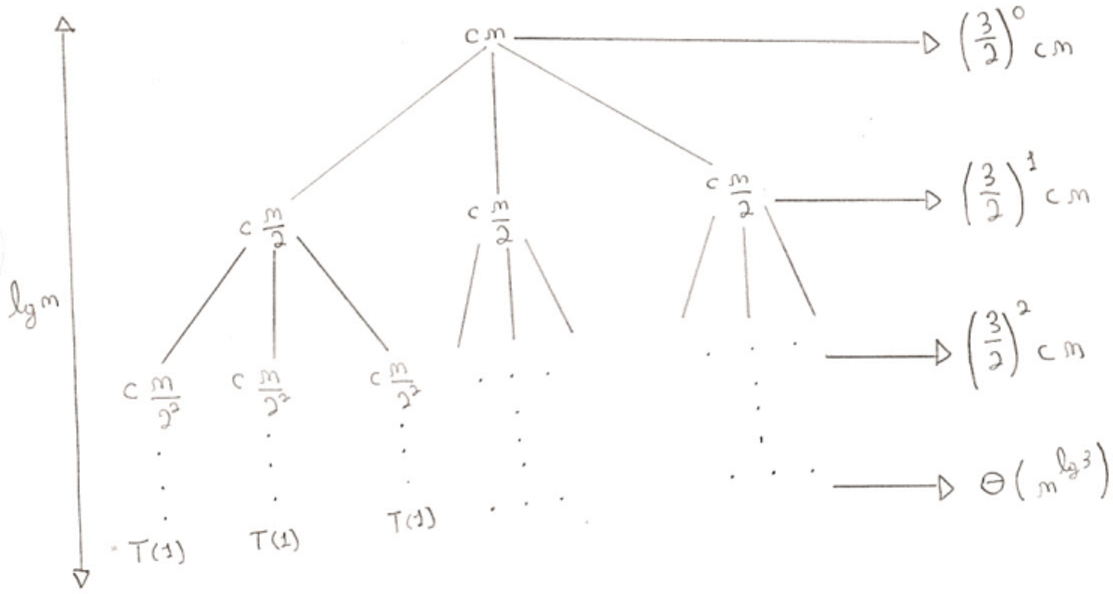
\includegraphics[width=0.7\textwidth]{images/4_4_1_1.pdf}
\end{center}

The number of nodes at depth $i$ is $3^i$. Since subproblem size reduce by
a factor of 2, each node at depth $i$, for $i = 0, 1, 2, \dots, \lg n - 1$,
has a cost of $c (n/2^i)$. Thus, the total cost over all nodes at depth
$i$, for $i = 0, 1, 2, \dots, \lg n - 1$, is $(3/2)^i cn$. The bottom level,
at deph $\lg n$, has $3^{\lg n} = n^{\lg 3}$ nodes, each contributing cost
$T(1)$, for a total cost of $n^{\lg 3} T(1) = \Theta(n^{\lg 3})$.

The cost of the entire tree is
\begin{equation*}
\begin{aligned}
T(n) &= cn + \frac{3}{2} cn + \left(\frac{3}{2}\right)^2 cn + \dots
           + \left(\frac{3}{2}\right)^{\lg n - 1} cn + \Theta\left({n^{\lg 3}}\right)\\
     &= \sum_{i = 0}^{\lg n - 1} \left(\frac{3}{2}\right)^i cn + \Theta(n^{\lg 3})\\
     &= cn \frac{\left(\frac{3}{2}\right)^{\lg n} - 1}{\frac{3}{2} - 1} + \Theta(n^{\lg 3})\\
     &= 2cn \left(\left(\frac{3}{2}\right)^{\lg n} - 1\right) + \Theta(n^{\lg 3})\\
     &= 2cn \frac{3^{\lg n}}{2^{\lg n}} - 2cn + \Theta(n^{\lg 3})\\
     &= 2cn \frac{n^{\lg 3}}{n} - 2cn + \Theta(n^{\lg 3})\\
     &= 2cn^{\lg 3} - 2cn + \Theta(n^{\lg 3})\\
     &= O(n^{\lg 3}).
\end{aligned}
\end{equation*}

Our guess is
\[
T(n) \le c n^{\lg 3} - dn \; \Forall n \ge n_0,
\]
where $c$, $d$, and $n_0$ are positive constants. Substituting into the
recurrence yields
\begin{equation*}
\begin{aligned}
  T(n) &\le 3 \left(c {\Bigl\lfloor\frac{n}{2}\Bigl\rfloor}^{\lg 3} - d {\Bigl\lfloor\frac{n}{2}\Bigl\rfloor}\right) + n\\
       &\le \frac{3c}{3} n^{\lg 3} - \frac{3d}{2}n + n\\
       &= c n^{\lg 3} - dn - \frac{d}{2}n + n\\
       &\le c n^{\lg 3} - dn,
\end{aligned}
\end{equation*}
where the last step holds as long as $d \ge 2$.
\end{framed}

\newpage

\item[4.4{-}2]{Use a recursion tree to determine a good asymptotic upper bound
on the recurrence $T(n) = T(n/2) + n^2$. Use the substitution method to verify
your answer.}

\begin{framed}
Figure below ilustrates the recursion tree $T(n) = T(n/2) + n^2$.

\begin{center}
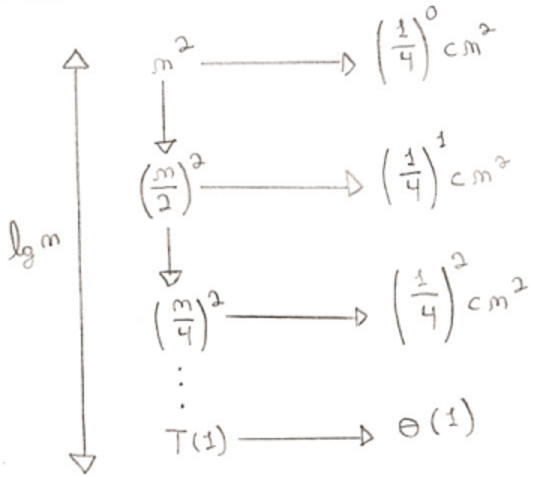
\includegraphics[width=0.3\textwidth]{images/4_4_2_1.pdf}
\end{center}

The tree has $\lg n$ levels and the cost at depth $i$ is
$c(n/2^i)^2 = (1/4)^i cn^2$.

The cost of the entire tree is
\begin{equation*}
\begin{aligned}
T(n) &= \sum_{i = 0}^{\lg n} \left(\frac{1}{4}\right)^i cn^2\\
     &< \sum_{i = 0}^{\infty} \left(\frac{1}{4}\right)^i cn^2\\
     &= \frac{1}{1 - (1/4)} cn^2\\
     &= \frac{4}{3} cn^2\\
     &= O(n^2).
\end{aligned}
\end{equation*}

Our guess is
\[
T(n) \le d n^2 \; \Forall n \ge n_0,
\]
where $d$, and $n_0$ are positive constants. Substituting into the
recurrence and using the same constant $c > 0$ as before yields
\begin{equation*}
\begin{aligned}
  T(n) &\le d \left(\frac{n}{2}\right)^2 + c n^2\\
       &= \frac{1}{4} dn^2 + cn^2\\
       &\le dn^2,
\end{aligned}
\end{equation*}
where the last step holds as long as $d \ge (4/3)c$.
\end{framed}

\newpage

\item[4.4{-}3]{Use a recursion tree to determine a good asymptotic upper bound
on the recurrence $T(n) = 4T(n/2 + 2) + n$. Use the substitution method to
verify your answer.}

\begin{framed}
Figure below ilustrates the recursion tree $T(n) = 4T(n/2 + 2) + n$.

\begin{center}
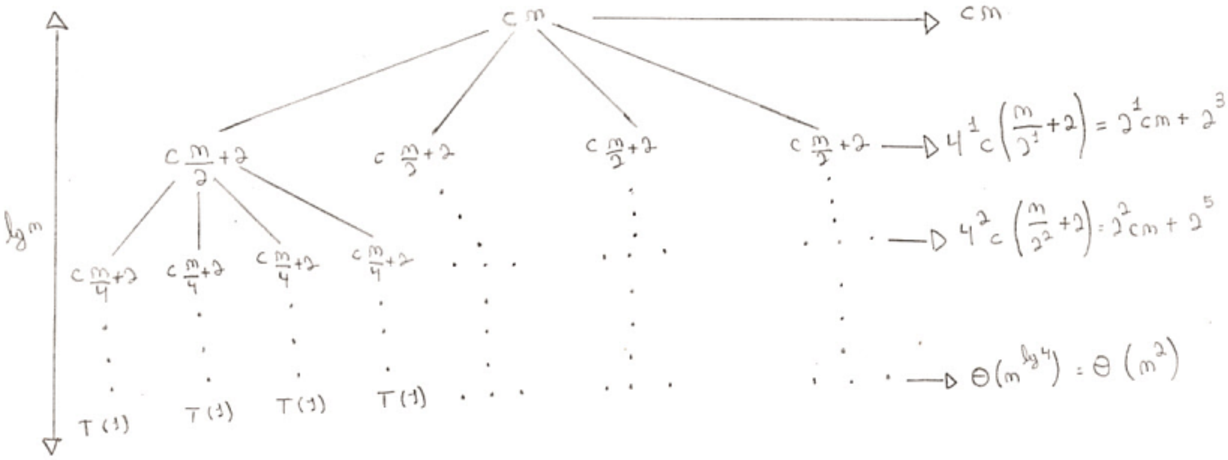
\includegraphics[width=0.9\textwidth]{images/4_4_3_1.pdf}
\end{center}

The number of nodes at depth $i$ is $4^i$. Since subproblem size reduce by
a factor of 2 and increment 2, each node at depth $i$, for
$i = 0, 1, 2, \dots, \lg n - 1$, has a cost of $c (n/2^i + 2)$. Thus, the total
cost over all nodes at depth $i$, for $i = 0, 1, 2, \dots, \lg n - 1$, is
$4^i c (n/2^i + 2) = 2^i cn + 2^{2i + 1}$. The bottom level, at deph $\lg n$,
has $4^{\lg n} = n^{\lg 4}$ nodes, each contributing cost $T(1)$, for a total
cost of $n^{\lg 4} T(1) = \Theta(n^{\lg 4})$.

The cost of the entire tree is
\begin{equation*}
\begin{aligned}
T(n) &= \sum_{i = 0}^{\lg n - 1} \left(4^i c \left(\frac{n}{2^i} + 2\right)\right) +
        \Theta(n^2)\\
     &= \sum_{i = 0}^{\lg n - 1} \left(4^i c \cdot \frac{n}{2^i}\right) +
        \sum_{i = 0}^{\lg n - 1} (4^i c \cdot 2) + \Theta(n^2)\\
     &= cn \sum_{i = 0}^{\lg n - 1} (2^i) + 2c \sum_{i = 0}^{\lg n - 1} (4^i) + \Theta(n^2)\\
     &= cn \frac{2^{\lg n} - 1}{2 - 1} + 2c \frac{4^{\lg n} - 1}{4 - 1} + \Theta(n^2)\\
     &= cn (n - 1) + \frac{2c}{3} (n^2 - 1) + \Theta(n^2)\\
     &= cn^2 - cn + \frac{2cn^2}{3} - \frac{2c}{3} + \Theta(n^2)\\
     &= O(n^2).
\end{aligned}
\end{equation*}

Our guess is
\[
T(n) \le c n^2 - dn \; \Forall n \ge n_0,
\]
where $c$, $d$, and $n_0$ are positive constants. Substituting into the
recurrence yields
\begin{equation*}
\begin{aligned}
  T(n) &\le 4 \left(c \left(\frac{n}{2} + 2\right)^2 - d\left(\frac{n}{2} + 2\right)\right) + n\\
       &\le 4 \left(c \frac{n^2}{4} + 2cn + 4c - \frac{dn}{2} - 2d\right) + n\\
       &= c n^2 + 8cn + 16c - 2dn - 8d + n\\
       &= c n^2 - dn - (d - 8c - 1)n - (d - 2c)8\\
       &\le c n^2 - dn,
\end{aligned}
\end{equation*}
where the last step holds as long as $d - 8c - 1 \ge 0$.
\end{framed}

\newpage

\item[4.4{-}4]{Use a recursion tree to determine a good asymptotic upper bound
on the recurrence $T(n) = 2T(n - 1) + 1$. Use the substitution method to verify
your answer.}

\begin{framed}
Figure below ilustrates the recursion tree $T(n) = 2T(n - 1) + 1$.

\begin{center}
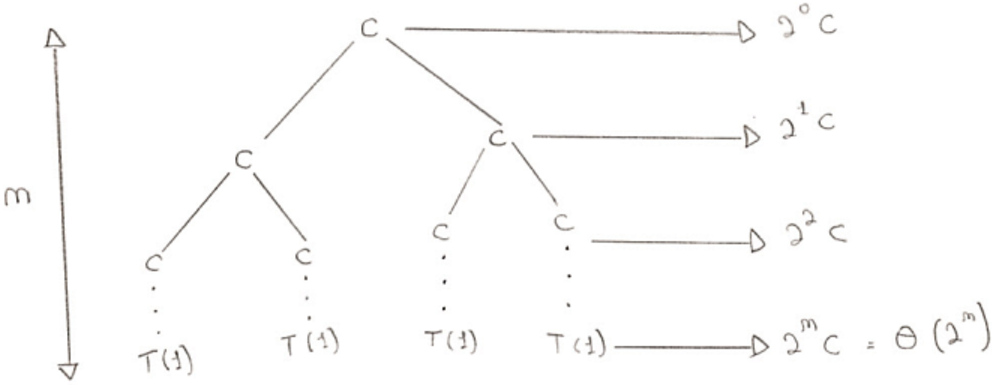
\includegraphics[width=0.6\textwidth]{images/4_4_4_1.pdf}
\end{center}

The tree has $n$ levels and $2^i$ nodes at each level. Since each node costs
$1$, the cost at depth $i$ is $2^i$. The bottom level, at deph $n$,
has $2^n$ nodes, each contributing cost $1$, for a total
cost of $2^n = \Theta(2^n)$.

The cost of the entire tree is
\begin{equation*}
\begin{aligned}
  T(n) &= \sum_{i = 0}^{n - 1} (2^i) + \Theta(2^n)\\
       &= \frac{2^n - 1}{2 - 1} + \Theta(2^n)\\
       &= 2^n - 1 + \Theta(2^n)\\
       &= O(2^n).
\end{aligned}
\end{equation*}

Our guess is
\[
T(n) \le c 2^n - d \; \Forall n \ge n_0,
\]
where $c$, $d$, and $n_0$ are positive constants. Substituting into the
recurrence yields
\begin{equation*}
\begin{aligned}
  T(n) &\le 2 (c 2^{n - 1} - d) + 1\\
       &= c2^n - 2d + 1\\
       &= c2^n - d - d + 1\\
       &\le c 2^n - d,
\end{aligned}
\end{equation*}
where the last step holds as long as $d \ge 1$.
\end{framed}

\newpage

\item[4.4{-}5]{Use a recursion tree to determine a good asymptotic upper bound
on the recurrence $T(n) = T(n - 1) + T(n/2) + n$. Use the substitution method to
verify your answer.}

\begin{framed}
Figure below ilustrates the recursion tree $T(n) = T(n - 1) + T(n/2) + n$.

\begin{center}
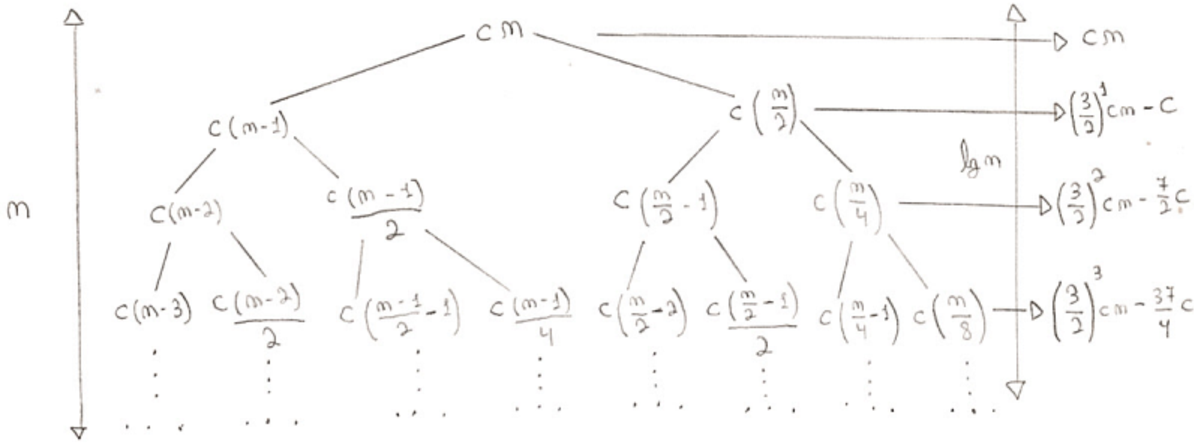
\includegraphics[width=0.85\textwidth]{images/4_4_5_1.pdf}
\end{center}

We start obtaining a lower bound. The cost of the initial levels (before level
$\lg n$) of the tree are
\[
cn \rightarrow (3/2)^1 cn - c \rightarrow (3/2)^2 cn - (7/2) c \rightarrow (3/2)^3 cn - (37/4) c.
\]

Thus, the cost of the tree from the root to level $\lg n$ is at most
\[
  \sum_{i = 0}^{\lg n} \left(\frac{3}{2}\right)^i cn
  = cn \frac{\left(\frac{3}{2}\right)^{\lg n + 1} - 1}{\frac{3}{2} - 1}
  = 2cn \frac{3}{2} \left(\frac{3}{2}\right)^{\lg n} - 2cn
  = 3cn \frac{n^{\lg 3}}{n} - 2cn
  = 3cn^{\lg 3} - 2cn
  = O(n^{\lg 3}).
\]

The cost of the longest simple path from the root to a leaf is
\[
  \sum_{i = 0}^{n} c(n - i) = c \sum_{i = 0}^{n} i = c \frac{n (n + 1)}{2}
                            = c \frac{n^2}{2} + \frac{c}{2} = O(n^2).
\]

Thus, our guess for a lower bound for $T(n)$ is
\[
T(n) \ge cn^2 \; \Forall n \ge n_0,
\]
where $c$, and $n_0$ are positive constants. Substituting into the
recurrence yields
\begin{equation*}
\begin{aligned}
  T(n) &\ge c (n - 1)^2 + c\left(\frac{n}{2}\right)^2 + n\\
       &=   cn^2 - 2cn + 1 + \frac{cn^2}{4} + n\\
       &=   \frac{5}{4} cn^2 -2cn + n + 1\\
       &\ge cn^2 -2cn + n + 1\\
       &\ge cn^2,
\end{aligned}
\end{equation*}
where the last step holds as long as $c \ge 1$ and $n_0 \ge 1$. Thus, we have
$T(n) = \Omega(n^2)$.

Consider now the recurrence
\[
S(n) = 2T(n - 1) + n,
\]
which is more costly than $T(n)$. We can easily prove that $S(n) = O(2^n)$. Our
guess for an upper bound of $S(n)$ is
\[
S(n) \le c 2^n - dn \; \Forall n \ge n_0,
\]
where $c$, $d$, and $n_0$ are positive constants. Substituting into the
recurrence yields
\begin{equation*}
\begin{aligned}
  S(n) &\le 2 (c 2^{n - 1} - d(n - 1)) + n\\
       &=   c2^n - 2dn + 2d + n\\
       &=   c2^n - dn - n(d - 1) + 2d\\
       &\le c 2^n - dn,
\end{aligned}
\end{equation*}
where the last step holds as long as $d \ge 2$ and $n_0 \ge 3$. Thus, we have
$T(n) = O(S(n)) = O(2^n)$.

We can obtain a more tight upper bound without using the recursion tree.
Let $R(n) = T(n/2) + n$. We have
\begin{equation*}
\begin{aligned}
  T(n) &= T(n - 1) + R(n)\\
       &= T(n - 2) + R(n - 1) + R(n)\\
       &= R(1) + R(2) + \dots + R(n - 1) + R(n)\\
       &\le n \cdot R(n)\\
       &= n \cdot T(n/2) + n^2,
\end{aligned}
\end{equation*}
which can be solved using the master method. We have $f(n) = n^2$ and
$n^{\log_b a} = n^{\lg n}$. Using the first case, we have
\[
f(n) = n^2 = O(n^{\lg n - \epsilon}), \; \text{($\epsilon = 1$)}
\]
which implies
\[
T(n) = O(n^{\lg n}).
\]
\end{framed}

\newpage

\item[4.4{-}6]{Argue that the solution to the recurrence
$T(n) = T(n/3) + T(2n/3) + cn$, where $c$ is a constant, is $\Omega(n \lg n)$ by
appealing to a recursion tree.}

\begin{framed}
Figure below ilustrates the recursion tree $T(n) = T(n/3) + T(2n/3) + cn$.

\begin{center}
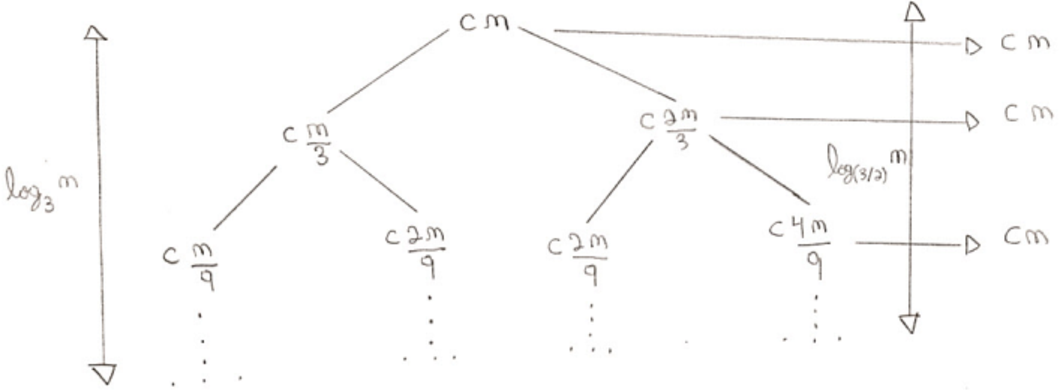
\includegraphics[width=0.7\textwidth]{images/4_4_6_1.pdf}
\end{center}

The tree is complete until level $\log_3 n$. The cost of the tree from the root
to level $\log_3 n$ is
\[
  \sum_{i = 0}^{\log_3 n} cn = cn \log_3 n,
\]
which is $\Omega(n \lg n)$.
\end{framed}

\newpage

\item[4.4{-}7]{Draw the recursion tree for $T(n) = 4T(\floor{n/2}) + cn$, where
$c$ is a constant, and provide a tight asymptotic bound on its solution. Verify
your bound by the substitution method.}

\begin{framed}
Since floors/ceiling usually do not matter, we will draw a recursion tree for
the recurrence $T(n) = 4T(n/2) + cn$.

\begin{center}
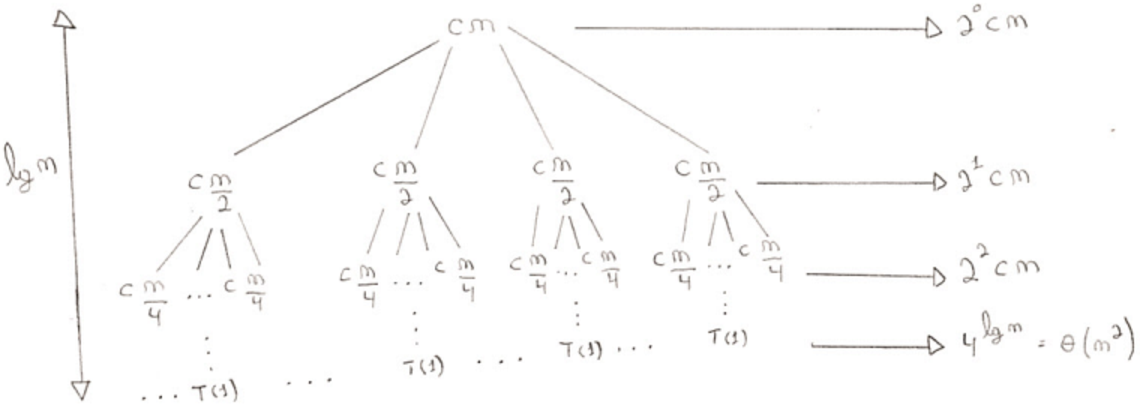
\includegraphics[width=0.9\textwidth]{images/4_4_7_1.pdf}
\end{center}

The number of nodes at depth $i$ is $4^i$. Since subproblem size reduce by
a factor of 2, each node at depth $i$, for $i = 0, 1, 2, \dots, \lg n - 1$,
has a cost of $c (n/2^i)$. Thus, the total cost over all nodes at depth
$i$, for $i = 0, 1, 2, \dots, \lg n - 1$, is $(4/2)^i cn = 2^i cn$. The bottom
level has $4^{\lg n} = n^2$ nodes, each contributing cost $T(1)$, for a total
cost of $n^2 T(1) = \Theta(n^2)$.

The cost of the entire tree is
\[
\sum_{i = 0}^{\lg n - 1} (2^i cn) + \Theta(n^2)
= cn \frac{2^{\lg n} - 1}{2 - 1} + \Theta(n^2)
= cn (n - 1) + \Theta(n^2)
= cn^2 - cn + \Theta(n^2)
= \Theta(n^2).
\]

Lets verify with the substitution method. Our guess for an upper bound is
\[
T(n) \le dn^2 - en \; \Forall n \ge n_0,
\]
where $d$, $e$, and $n_0$ are positive constants. Substituting into the
recurrence yields
\begin{equation*}
\begin{aligned}
  T(n) &\le 4\left(d \Bigl\lfloor\frac{n}{2}\Bigl\rfloor^2 -e \frac{n}{2}\right) + cn\\
       &\le 4\left(d \left(\frac{n}{2}\right)^2 -e \frac{n}{2}\right) + cn\\
       &=   4\left(d \frac{n^2}{4} -e \frac{n}{2}\right) + cn\\
       &=   d n^2 -2en + cn\\
       &=   d n^2 - en - en + cn\\
       &\le   d n^2 - en,
\end{aligned}
\end{equation*}
where the last step holds as long as $e \ge c$.

Our guess for a lower bound is
\[
T(n) \ge dn^2 \; \Forall n \ge n_0,
\]
where $d$, and $n_0$ are positive constants. Substituting into the
recurrence yields
\begin{equation*}
\begin{aligned}
  T(n) &\ge 4d \Bigl\lfloor\frac{n}{2}\Bigl\rfloor^2 + cn\\
       &\ge 4d \left(\frac{n}{2} - 1\right)^2 + cn\\
       &=   4d \left( \frac{n^2}{4} - n + 1 \right) + cn\\
       &=   d n^2 - 4dn + 4d + cn\\
       &=   d n^2 - (4d - c)n + 4d
\end{aligned}
\end{equation*}
where the last step holds as long as $4d - c \ge 4$ and $n_0 \ge d$.
\end{framed}

\newpage

\item[4.4{-}8]{Use a recursion tree to give an asymptotically tight solution to
the recurrence $T(n) = T(n - a) + T(a) + cn$, where $a \ge 1$ and $c > 0$ are
constants.}

\begin{framed}
Figure below ilustrates the recursion tree $T(n) = T(n - a) + T(a) + cn$.

\begin{center}
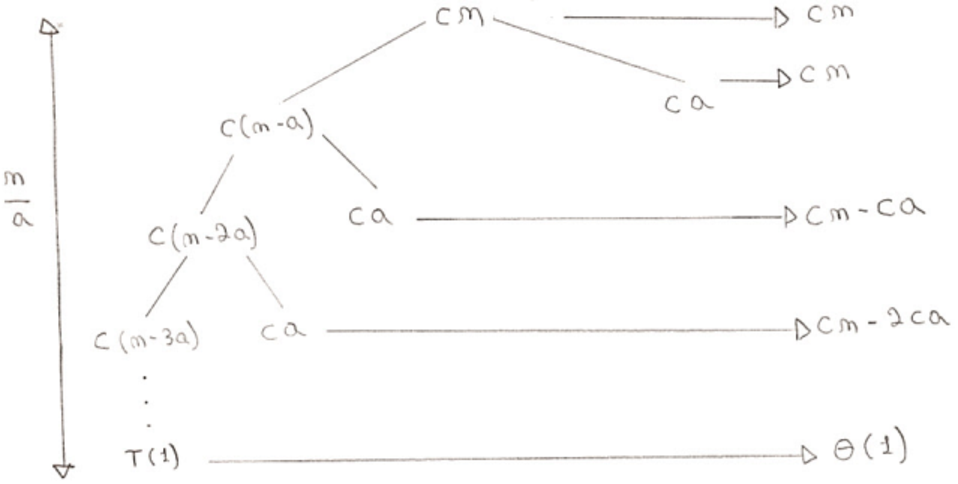
\includegraphics[width=0.7\textwidth]{images/4_4_8_1.pdf}
\end{center}

The height of the tree is $n/a$. Each level $i$, for $i = 1, 2, \dots, (n/a)$,
has two nodes, one that costs $c(n - ia)$ and another that costs $T(a) = ca$.
Thus, the cost over the nodes at depth $i$, for $i = 1, 2, \dots, (n/a)$, is
$c(n - a) + ca$. The root level, at deph 0, has a single node that costs $cn$.

The cost of the entire tree is
\begin{equation*}
\begin{aligned}
  T(n) &= cn + \sum_{i = 1}^{n/a} (c (n - ia) + ca)\\
       &= cn + \sum_{i = 1}^{n/a} cn - \sum_{i = 1}^{n/a} cia + \sum_{i = 1}^{n/a} ca\\
       &= cn + c\frac{n^2}{a} - \frac{cn (a + n)}{2a} + cn\\
       &= c \frac{n^2}{a} - c\frac{n^2}{2a} - c \frac{n}{2} + 2cn\\
       &= c \frac{n^2}{2a} + \frac{3}{2} cn\\
       &= \Theta(n^2).
\end{aligned}
\end{equation*}

Lets verify with the substitution method. Our guess for an upper bound is
\[
T(n) \le cn^2 \; \Forall n \ge n_0,
\]
where $c$ and $n_0$ are positive constants. Substituting into the
recurrence yields
\begin{equation*}
\begin{aligned}
  T(n) &\le c (n^2 - 2an + a^2) + ca + cn\\
       &=   cn^2 - c (2an - a - n - a^2)\\
       &\le cn^2,
\end{aligned}
\end{equation*}
where the last step holds as long as $n_0 \ge a$.

Our guess for a lower bound is
\[
  T(n) \ge \frac{c}{2a} n^2 \; \Forall n \ge n_0,
\]
where $c$, and $n_0$ are positive constants. Substituting into the
recurrence yields
\begin{equation*}
\begin{aligned}
  T(n) &\ge \frac{c}{2a} (n - a)^2 + ca + cn\\
       &=   \frac{c}{2a} (n^2 - 2an + a^2) + ca + cn\\
       &=   \frac{c}{2a} n^2 - cn + \frac{1}{2} ca + ca + cn\\
       &=   \frac{c}{2a} n^2 + \frac{3}{2} ca\\
       &\ge \frac{c}{2a} n^2.
\end{aligned}
\end{equation*}
\end{framed}

\newpage

\item[4.4{-}9]{Use a recursion tree to give an asymptotically tight solution to
the recurrence $T(n) = T(\alpha n) + T((1 - \alpha) n) + cn$, where $\alpha$ is
a constant in the range $0 < \alpha < 1$ and $c > 0$ is also a constant.}

\begin{framed}
Let $\alpha \ge 1 - \alpha$. Figure below ilustrates the recursion tree
$T(n) = T(\alpha n) + T((1 - \alpha n) n) + cn$.

\begin{center}
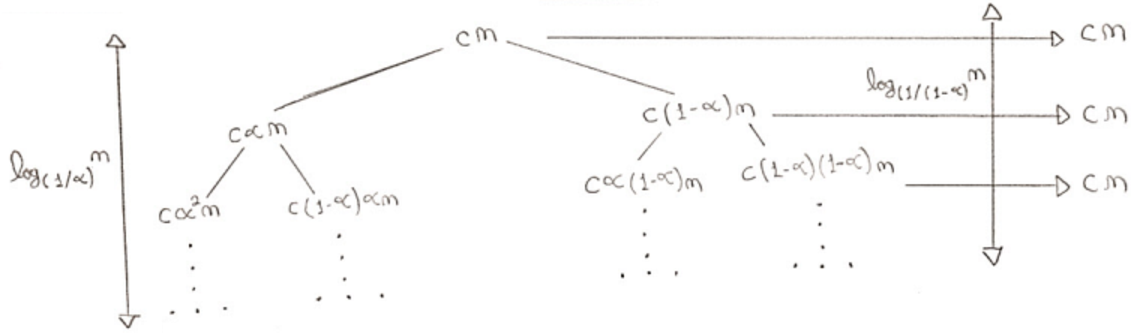
\includegraphics[width=0.8\textwidth]{images/4_4_9_1.pdf}
\end{center}

If it were a complete tree, all the $\log_{1 - \alpha} n$ levels would cost $cn$
and the entire tree $cn \log_{1 - \alpha} n$. Thus,
$T(n) = O(n \log_{1 - \alpha} n) = O(n \lg n)$. The tree is complete until level
$\log_{1/(1 - \alpha)} n$. The cost of the tree from the root to level
$\log_{1/(1 - \alpha)} n$ is
\[
  \sum_{i = 0}^{\log_{1/(1 - \alpha)} n} cn
  = \left(\sum_{i = 1}^{\log_{1/(1 - \alpha)} n} cn\right) + cn
  = cn (\log_{1/(1 - \alpha)} n) + cn,
\]
which is $\Omega(n \log_{1/(1 - \alpha)} n)$ = $\Omega(n \lg n)$.

Lets verify with the substitution method. Our guess for an upper bound is
\[
T(n) \le d n \lg n \; \Forall n \ge n_0,
\]
where $d$ and $n_0$ are positive constants. Substituting into the
recurrence yields
\begin{equation*}
\begin{aligned}
  T(n) &\le d \alpha n \lg (\alpha n) + d (1 - \alpha) n \lg ((1 - \alpha) n) + dn\\
       &=   d \alpha n \lg \alpha + d \alpha n \lg n + d (1 - \alpha) n \lg (1 - \alpha) + d (1 - \alpha) n \lg n + cn\\
       &=   d \alpha n \lg \alpha + d \alpha n \lg n + d (1 - \alpha) n \lg (1 - \alpha) + d n \lg n - d \alpha n \lg n + cn\\
       &=   d n \lg n + dn (\alpha \lg \alpha + (1 - \alpha) \lg (1 - \alpha)) + cn\\
       &\le d n \lg n,
\end{aligned}
\end{equation*}
where the last step holds as long as $d(\alpha \lg \alpha + (1 - \alpha) \lg (1 - \alpha)) + c \le 0$.

Our guess for a lower bound is
\[
  T(n) \ge d n \lg n \; \Forall n \ge n_0,
\]
where $d$, and $n_0$ are positive constants. Substituting into the
recurrence yields
\begin{equation*}
\begin{aligned}
  T(n) &\ge d \alpha n \lg (\alpha n) + d (1 - \alpha) n \lg ((1 - \alpha) n) + dn\\
       &=   d \alpha n \lg \alpha + d \alpha n \lg n + d (1 - \alpha) n \lg (1 - \alpha) + d (1 - \alpha) n \lg n + cn\\
       &=   d \alpha n \lg \alpha + d \alpha n \lg n + d (1 - \alpha) n \lg (1 - \alpha) + d n \lg n - d \alpha n \lg n + cn\\
       &=   d n \lg n + dn (\alpha \lg \alpha + (1 - \alpha) \lg (1 - \alpha)) + cn\\
       &\ge d n \lg n,
\end{aligned}
\end{equation*}
where the last step holds as long as $d(\alpha \lg \alpha + (1 - \alpha) \lg (1 - \alpha)) + c \ge 0$.
\end{framed}

\end{enumerate}

\newpage

\section{The master method for solving recurrences}

\begin{enumerate}

\item[4.5{-}1]{Use the master method to give tight asymptotic bounds for the
following recurrences.

\begin{enumerate}
  \item[a.] $T(n) = 2T(n/4) + 1$.
  \item[b.] $T(n) = 2T(n/4) + \sqrt{n}$.
  \item[c.] $T(n) = 2T(n/4) + n$.
  \item[d.] $T(n) = 2T(n/4) + n^2$.
\end{enumerate}
}

\begin{framed}
\begin{enumerate}
  \item[(a)] Case 1 applies. $T(n) = \Theta(n^{\log_4{2}}) = \Theta(\sqrt{n})$.
  \item[(b)] Case 2 applies. $T(n) = \Theta(n^{\log_4{2}} \lg n) = \Theta(\sqrt{n} \lg n)$.
  \item[(c)] Case 3 applies. $T(n) = \Theta(n)$.
  \item[(d)] Case 3 applies. $T(n) = \Theta(n^2)$.
\end{enumerate}
\end{framed}

\item[4.5{-}2]{Professor Caesar wishes to develop a matrix-multiplication
algorithm that is asymptotically faster than Strassen's algorithm. His algorithm
will use the divide-and-conquer method, dividing each matrix into pieces of
size $n/4 \times n/4$, and the divide and combine steps together will take
$\Theta(n^2)$ time. He needs to determine how many subproblems his algorithm has
to create in order to beat Strassen's algorithm. If his algorithm creates $a$
subproblems, then the recurrence for the running time $T(n)$ becomes
$T(n) = a T(n/4) + \Theta(n^2)$. What is the largest integer value of $a$ for
which Professor Caesar's algorithm would be asymptotically faster than
Strassen's algorithm?}

\begin{framed}
Strassen's algorithm costs $\Theta(n^{\lg 7})$. The cost of $T(n)$ is stated
below.
\begin{itemize}
  \item If $a < 16$, Case 3 applies. $T(n) = \Theta(n^2) = o(n^{\lg 7})$.
  \item If $a = 16$, Case 2 applies. $T(n) = \Theta(n^2 \lg n) = o(n^{\lg 7})$.
  \item If $a > 16$, Case 1 applies. $T(n) = \Theta(n^{\log_4{a}}) = o(n^{\lg 7})$ when $a < 49$.
\end{itemize}
Thus, the largest integer value of $a$ is 48.
\end{framed}

\item[4.5{-}3]{Use the master method to show that the solution to the
binary-search recurrence $T(n) = T(n/2) + \Theta(1)$ is $T(n) = \Theta(\lg n)$.
(See Exercise 2.3-5 for a description of binary search.)}

\begin{framed}
We have
\[
n^{\log_b a} = n^{\lg 1} = \Theta(1) = f(n).
\]
Thus, Case 2 applies. $T(n) = \Theta(\lg n)$.
\end{framed}

\newpage

\item[4.5{-}4]{Can the master method be applied to the recurrence
$T(n) = 4 T(n/2) + n^2 \lg n$? Why or why not? Give an asymptotic upper bound
for this recurrence.}

\begin{framed}
We have
\[
  f(n) = n^2 \lg n,
\]
and
\[
n^{\log_b a} = n^{\log_2 4} = \Theta(n^2),
\]
which is larger than $f(n)$, but not polynomially larger. Thus, we cannot use the
master method to solve this recurrence.

We can use a recursion tree to guess the cost of $T(n)$ and verify with the
substitution method. Figure below ilustrates the recursion tree of
$T(n) = 4 T(n/2) + n^2 \lg n$.

\begin{center} Figure here. \end{center}

The tree has $\lg n$ levels and the number of nodes at depth $i$ is $4^i$. Each
node at depth $i$ has a cost $c((n/2^i)^2) \lg(n) = 1/4^i c n^2 \lg n$. Thus,
the total cost at depth $i$ is $4^i \times 1/4^i c n^2 \lg n = c n^2 \lg n$.

The cost of the entire tree is
\[
  \sum_{i = 0}^{\lg n} c n^2 \lg n = O(n^2 \lg^2 n).
\]

Lets verify with the substitution method. Our guess is
\[
T(n) \le cn^2\lg^2 n \; \Forall n \ge n_0,
\]
where $c$ and $n_0$ are positive constants. Substituting into the
recurrence yields
\begin{equation*}
\begin{aligned}
  T(n) &\le 4c \left(\left(\frac{n}{2}\right)^2 \lg^2{\left(\frac{n}{2}\right)}\right) + n^2 \lg n\\
       &=   4c \left(\frac{n^2}{4} \lg{\left(\frac{n}{2}\right)}\lg{\left(\frac{n}{2}\right)}\right) + n^2 \lg n\\
       &=   c n^2 \lg{\left(\frac{n}{2}\right)}\lg{\left(\frac{n}{2}\right)} + n^2 \lg n\\
       &=   c n^2 \lg{\left(\frac{n}{2}\right)}\lg n - c n^2 \lg{\left(\frac{n}{2}\right)} + n^2 \lg n\\
       &=   c n^2 \lg^2 n - c n^2 \lg n - c n^2 \lg n + c n^2 + n^2 \lg n\\
       &\le c n^2 \lg^2 n,
\end{aligned}
\end{equation*}
where the last step holds as long as $c \ge 1$.

\end{framed}

\item[4.5{-}5]{Consider the regularity condition $a f(n/b) \ge c f(n)$ for some
constant $c < 1$, which is part of case 3 of the master theorem. Give an example
of constants $a \ge 1$ and $b > 1$ and a function $f(n)$ that satisfies all
the conditions in case 3 of the master theorem except the regularity
condition.}

\begin{framed}
Let $a = 1$, $b = 2$, and $f(n) = n \cos n$. We have
\[
  n^{\log_b a} = n^{\log_2 1} = \Theta(1),
\]
which is polynomially smaller than $f(n)$ and satisfies the primary condition of
Case 3. However, we have
\[
  a f\left(\frac{n}{b}\right) \le c f(n) \rightarrow \frac{n}{2} \cos\left(\frac{n}{2}\right) \le c ( n \cos n ),
\]
which is not valid for some constant $c < 1$ and all sufficiently large $n$
since $\cos(\cdot)$ is not monotonic. Thus, it satisfies the primary condition
of Case 3, but not the regularity condition
\end{framed}

\end{enumerate}

\newpage

\section*{Problems}
\addcontentsline{toc}{section}{\protect\numberline{}Problems}%

\begin{enumerate}

\item[4{-}1]{\textbf{\emph{Recurrence examples}}\\
Give asymptotic upper and lower bounds for $T(n)$ in each of the following
recurrences. Assume that $T(n)$ is constant for $n \ge 2$. Make your bounds as
tight as possible, and justify your answers.

\begin{enumerate}
  \item [a.] $2T(n/2) + n^4$.
  \item [b.] $T(7n/10) + n$.
  \item [c.] $16T(n/4) + n^2$.
  \item [d.] $7T(n/3) + n^2$.
  \item [e.] $7T(n/2) + n^2$.
  \item [f.] $2T(n/4) + \sqrt{n}$.
  \item [g.] $T(n - 2) + n^2$.
\end{enumerate}
}

\begin{framed}
\begin{enumerate}
  \item[(a)] We use the master method. Case 3 applies, since $n^{\lg 2} = n$ is
    polynomially smaller than $f(n)$. Thus, $T(n) = \Theta(n^4)$.
  \item[(b)] We use the master method. Case 3 applies, since
    $n^{\log_{10/7} 1} = 1$ is polynomially smaller than $f(n)$. Thus,
    $T(n) = \Theta(n)$.
  \item[(c)] We use the master method. Case 2 applies, since
    $n^{\log_4 14} = n^2 = \Theta(f(n))$. Thus, $T(n) = \Theta(n^2 \lg n)$.
  \item[(d)] We use the master method. Case 3 applies, since $n^{\log_3 7}$ is
    polynomially smaller than $f(n)$. Thus, $T(n) = \Theta(n^2)$.
  \item[(e)] We use the master method. Case 1 applies, since $n^{\lg 7}$ is
    polynomially larger than $f(n)$. Thus, $T(n) = \Theta(n^{\lg 7})$.
  \item[(f)] We use the master method. Case 2 applies, since
    $n^{\log_4 2} = \sqrt n = \Theta(f(n))$. Thus, $T(n) = \Theta(\sqrt n \lg n)$.
  \item[(g)] The recurrence has $n/2$ levels and depth $i$ costs $c(n - 2i)^2$.
    Thus, we have
    \[
      T(n) = \sum_{i = 0}^{n/2} c(n - 2i)^2
           = \sum_{i = 0}^{n/2} c(n^2 - 4ni + 4i^2)
           = c \left(\sum_{i = 0}^{n/2} n^2 - \sum_{i = 0}^{n/2} 4ni + \sum_{i = 0}^{n/2} 4i^2\right)
           = \Theta(n^3) - \Theta(n^2) + \Theta(n^3)
           = \Theta(n^3).
    \]
\end{enumerate}
\end{framed}

\newpage

\item[4{-}2]{\textbf{\emph{Parameter-passing costs}}\\
Throughout this book, we assume that parameter passing during procedure calls
takes constant time, even if an $N$-element array is being passed. This
assumption is valid in most systems because a pointer to the array is passed,
not the array itself.  This problem examines the implications of three
parameter-passing strategies:

\begin{enumerate}
  \item[1.] An array is passed by pointer. Time = $\Theta(1)$.
  \item[2.] An array is passed by copying. Time = $\Theta(N)$, where $N$ is the size
    of the array.
  \item[3.] An array is passed by copying only the subrange that might be accessed
    by the called procedure. Time = $\Theta(q - p + 1)$ if the subarray $A[p
    \dots q]$ is passed.
\end{enumerate}

\begin{enumerate}
  \item[a.] Consider the recursive binary search algorithm for finding a number
    in a sorted array (see Exercise 2.3-5). Give recurrences for the worst-case
    running times of binary search when arrays are passed using each of the
    three methods above, and give good upper bounds on the solutions of the
    recurrences. Let $N$ be the size of the original problem and $n$ be the size
    of a subproblem.
  \item[b.] Redo part (a) for the \textsc{Merge-Sort} algorithm from Section
    2.3.1.
\end{enumerate}
}

\begin{framed}
  \begin{enumerate}
    \item[a.] Binary search.
      \begin{enumerate}
        \item[1.] \emph{Array passed by pointer.}\\
          $T(n) = T(n/2) + \Theta(1)$.
          Case 2 of master method applies, since
          $n^{\lg 1} = 1 = f(n)$. Thus, $T(n) = \Theta(\lg n)$.
        \item[2.] \emph{Array passed by copying.}\\
          $T(n) = T(n/2) + \Theta(N) = T(n/4) + \Theta(N) + \Theta(N)$
          $= T(n/8) + \Theta(N) + \Theta(N) + \Theta(N)$
          $= \dots = \sum_{i = 0}^{\lg n} \Theta(N) = \Theta(n \lg n)$.
        \item[3.] \emph{Subarray passed by copying.}\\
          $T(n) = T(n/2) + \Theta(n)$.
          Case 3 of master method applies, since $n^{\lg 1} = 1$ is
          polynomially smaller than $f(n)$.\\
          Thus, $T(n) = \Theta(n)$.
      \end{enumerate}
    \item[b.] Merge sort.
      \begin{enumerate}
        \item[1.] \emph{Array passed by pointer.}\\
          $T(n) = T(\floor{n/2}) + T(\ceil{n/2}) + \Theta(n) \approx 2T(n/2) + \Theta(n)$.
          Case 2 of master method applies, since
          $n^{\lg 2} = n = f(n)$. Thus, $T(n) = \Theta(n \lg n)$.
        \item[2.] \emph{Array passed by copying.}\\
          $T(n) = 2T(n/2) + \Theta(N) = 4T(n/4) + 2\Theta(N) + \Theta(N)$
          $= 16T(n/8) + 4\Theta(N) + 2\Theta(N) + \Theta(N)$
          $= \dots = \sum_{i = 0}^{\lg n} 2^i \Theta(N) = \Theta(n^2)$.
        \item[3.] \emph{Subarray passed by copying.}\\
          $T(n) = 2T(n/2) + \Theta(n)$.
          Case 2 of master method applies, since
          $n^{\lg 2} = n = f(n)$. Thus, $T(n) = \Theta(n \lg n)$.
      \end{enumerate}
  \end{enumerate}
\end{framed}

\newpage

\item[4{-}3]{\textbf{\emph{More recurrence examples}}\\
Give asymptotic upper and lower bounds for $T(n)$ in each of the following
recurrences. Assume that $T(n)$ is constant for sufficiently small $n$. Make
your bounds as tight as possible, and justify your answers.

\begin{enumerate}
  \item[a.] $T(n) = 4T(n/3) + n \lg n$.
  \item[b.] $T(n) = 3T(n/3) + n / \lg n$.
  \item[c.] $T(n) = 4T(n/2) + n^2 \sqrt n$.
  \item[d.] $T(n) = 3T(n/3 - 2) + n/2$.
  \item[e.] $T(n) = 2T(n/2) + n / \lg n$.
  \item[f.] $T(n) = T(n/2) + T(n/4) + T(n/8) + n$.
  \item[g.] $T(n) = T(n - 1) + 1/n$.
  \item[h.] $T(n) = T(n - 1) + \lg n$.
  \item[i.] $T(n) = T(n - 2) + 1 / \lg n$.
  \item[j.] $T(n) = \sqrt n T(\sqrt n) + n$.
\end{enumerate}
}

\begin{framed}
  \begin{enumerate}
    \item[a.] We have $f(n) = n \lg n$ and $n^{\lg_b a} = n^{\log_3 4}$.
      Since $n \lg n = O(n^{\log_3(4) - 0.2})$, case 1 applies and we have
      $T(n) = \Theta(n^{\log_3 4})$.
    \item[b.] The tree has $\log_3 n$ levels and depth $i$, for $i = 0, 1,
      \dots, \log_3 n - 1$, costs $n/(\log_3 n - i)$. The cost of the entire
      tree is
      \[
        T(n) = \sum_{i = 0}^{\log_3 n - 1} \frac{n}{\log_3 n - i}
             = \sum_{i = 1}^{\log_3 n} \frac{n}{i}
             = n \sum_{i = 1}^{\log_3 n} \frac{1}{i}
             = n \cdot H_{\log_3 n}
             = n \cdot \Theta(\lg \log_3 n)
             = \Theta(n \lg \lg n).
      \]
      Skipped the proof.
    \item[c.] We have $f(n) = n^2 \sqrt n = n^{5/2}$ and
      $n^{\log_b a} = n^{\log_2 4} = n^2$. Since
      $n^{5/2} = \Omega(n^{2 + 1/2})$, we look at the regularity condition in
      case 3 of the master method. We have
      $af(n/b) = 4(n/2)^2 \sqrt{n/2} = (n^{5/2})/\sqrt 2 \le c n^{5/2}$ for
      $1/\sqrt 2 \le c < 1$. Case 3 applies and we have
      $T(n) = \Theta(n^2 \sqrt n)$.
    \item[d.]
      The tree has $\log_3 n$ levels and depth $i$, for
      $i = 0, 1, \dots, \log_3 n - 1$ costs $c (n/2) - 2 \cdot 3^i$. The cost of
      the entire tree is
      \[
        T(n) = \sum_{i = 0}^{\log_3 n - 1} \left(c \frac{n}{2} - 2 \cdot 3^i\right)
             = c \sum_{i = 0}^{\log_3 n - 1} \frac{n}{2} - 2 \sum_{i = 0}^{\log_3 n - 1} 3^i
             = \Theta(n \lg n).
      \]
      Our guess for the upper bound is
      \[
      T(n) \le c n \lg n \; \Forall n \ge n_0,
      \]
      where $c$ and $n_0$ are positive constants. Substituting into the recurrence
      yields
      \begin{equation*}
      \begin{aligned}
        T(n) &\le 3c \left(\frac{n}{3} - 2\right) \lg \left(\frac{n}{3} - 2\right) + \frac{n}{2}\\
             &=   c n \lg \left(\frac{n}{3} - 2\right) - 6c \lg \left(\frac{n}{3} - 2\right) + \frac{n}{2}\\
             &\le cn \lg \left(\frac{n}{3} - 2\right) - 6c \lg \left(\frac{n}{4}\right) + \frac{n}{2} & \text{($n \ge 24$)}\\
             &=   cn \lg \left(\frac{n}{3} - 2\right) - 6c \lg n - 12 c + \frac{n}{2}\\
             &<   cn \lg n - 6c \lg n - 12c + \frac{n}{2}\\
             &\le cn \lg n,
      \end{aligned}
      \end{equation*}
      where the last step holds as long as $-6c \lg n - 12c + n/2 \le 0$
      (skipped simplification).

      Our guess for the lower bound is
      \[
      T(n) \ge c n \lg n \; \Forall n \ge n_0,
      \]
      where $c$, and $n_0$ are positive constants. Substituting into the recurrence
      yields
      \begin{equation*}
      \begin{aligned}
        T(n) &\ge 3c \left(\frac{n}{3} - 2\right) \lg \left(\frac{n}{3} - 2\right) + \frac{n}{2}\\
             &=   c n \lg \left(\frac{n}{3} - 2\right) - 6c \lg \left(\frac{n}{3} - 2\right) + \frac{n}{2}\\
             &\ge cn \lg \left(\frac{n}{4}\right) - 6c \lg \left(\frac{n}{3} - 2\right) + \frac{n}{2} & \text{($n \ge 24$)}\\
             &=   cn \lg n - 2cn - 6c \lg \left(\frac{n}{3} - 2\right) + \frac{n}{2}\\
             &\ge cn \lg n,
      \end{aligned}
      \end{equation*}
      where the last step holds as long as $-2cn - 6c \lg (n/3 - 2) + n/2 \ge 0$
      (skipped simplification).
    \item[e.] The tree has $\lg n$ levels and depth $i$, for $i = 0, 1,
      \dots, \lg n - 1$, costs $n/(\lg n - i)$. The cost of the entire
      tree is
      \[
        T(n) = \sum_{i = 0}^{\lg n - 1} \frac{n}{\lg n - i}
             = \sum_{i = 1}^{\lg n} \frac{n}{i}
             = n \sum_{i = 1}^{\lg n} \frac{1}{i}
             = n \cdot H_{\lg n}
             = n \cdot \Theta(\lg \lg n)
             = \Theta(n \lg \lg n).
      \]
      Skipped the proof.
    \item[f.] The tree has $\lg n$ levels, but is not complete. Considering
      only the levels in which the tree is complete, depth $i$, for
      $i = 1, 2, \dots, \log_8 n$, costs $(7/8)^i cn$. Thus, the cost of the
      entire tree is at most
      \[
        T(n) \le \sum_{i=0}^{\lg n - 1} \left( \left(\frac{7}{8}\right)^i cn \right)
             = cn \sum_{i=0}^{\lg n - 1} \left( \left(\frac{7}{8}\right)^i \right)
             = cn \frac{1 - \left(\frac{7}{8}\right)^{\lg n}}{1 - \frac{7}{8}}
             = cn \frac{1 - n^{\lg 7 - 3}}{\frac{1}{8}}
             = 8cn - 8cn^{\lg 7 - 2}
             = O(n).
      \]
      Our guess for the upper bound is
      \[
      T(n) \le c n \; \Forall n \ge n_0,
      \]
      where $c$ and $n_0$ are positive constants. Substituting into the recurrence
      yields
      \begin{equation*}
      \begin{aligned}
        T(n) &\le c \frac{n}{2} + c \frac{n}{4} + c \frac{n}{8}\\
             &= \frac{7}{8} cn + n\\
             &\le cn,
      \end{aligned}
      \end{equation*}
      where the last step holds as long as $c \ge 8$.

      Our guess for the lower bound is
      \[
      T(n) \ge c n \; \Forall n \ge n_0,
      \]
      where $c$ and $n_0$ are positive constants. Substituting into the recurrence
      yields
      \begin{equation*}
      \begin{aligned}
        T(n) &\ge c \frac{n}{2} + c \frac{n}{4} + c \frac{n}{8}\\
             &= \frac{7}{8} cn + n\\
             &\ge cn,
      \end{aligned}
      \end{equation*}
      where the last step holds as long as $c \le 8$.
    \item[g.] The tree has $n$ levels and depth $i$, for
      $i = 1, 2, \dots, n - 1$, costs $1/(n - i)$. The cost of the entire tree
      is
      \[
        \sum_{i = 0}^{n - 1} \frac{1}{n - i} = \sum_{i = 1}^{n} \frac{1}{i} = H_n = \Theta(\lg n).
      \]
      Skipped the proof.
    \item[h.] The tree has $n$ levels and depth $i$, for
      $i = 1, 2, \dots, n - 1$, costs $\lg(n - i)$. The cost of the entire tree
      is
      \[
        \sum_{i = 0}^{n - 1} \lg(n - i) = \sum_{i = 1}^{n} \lg i = \lg(n!) = \Theta(n \lg n).
      \]
      Skipped the proof.
    \item[i.] Skipped.
    \item[j.] Skipped.
  \end{enumerate}
\end{framed}

\newpage

\item[4{-}4]{\textbf{\emph{Fibonacci numbers}}\\
This problem develops properties of the Fibonacci numbers, which are defined by
recurrence (3.22). We shall use the technique of generating functions to solve
the Fibonacci recurrence. Define the generating function (or formal power
series) $\mathcal{F}$ as

\begin{equation*}
\begin{aligned}
  \mathcal{F}(z) &= \sum_{i = 0}^\infty F_i z^i
                 &= 0 + z + z^2 + 2z^3 + 3z^4 + 5z^5 + 8z^6 + 13z^7 + 21z^8 + \dots,
\end{aligned}
\end{equation*}
where $F_i$ is the $i$th Fibonacci number.

\begin{enumerate}
  \item[a.] Show that $\mathcal{F}(z) = z + z \mathcal{F}(z) + z^2 \mathcal{F}(z)$.
  \item[b.] Show that
    \begin{equation*}
    \begin{aligned}
      \mathcal{F}(z) &= \frac{z}{1 - z - z^2}\\
                     &= \frac{z}{(1 - \phi z)(1 - \hat\phi z)}\\
                     &= \frac{1}{\sqrt 5} \left( \frac{1}{1 - \phi z} - \frac{1}{1 - \hat\phi z} \right),
    \end{aligned}
    \end{equation*}
    where
    \[
      \phi = \frac{1 + \sqrt 5}{2} = 1.61803 \dots
    \]
    and
    \[
      \hat\phi = \frac{1 - \sqrt 5}{2} = 0.61803 \dots .
    \]
  \item[c.] Show that
    \begin{equation*}
    \begin{aligned}
      \mathcal{F}(z) &= \sum_{i = 0}^\infty \frac{1}{\sqrt 5} (\phi^i - \hat\phi^i) z^i.
    \end{aligned}
    \end{equation*}
  \item[d.] Use part (c) to prove that $F_i = \phi^i/\sqrt{5}$ for $i > 0$,
    rounded to the nearest integer.\\(Hint: Observe that $|\hat\phi| < 1$.)
\end{enumerate}
}

\begin{framed}
  \begin{enumerate}
    \item[a.]
      \begin{equation*}
      \begin{aligned}
        \mathcal{F}(z) &= \sum_{i = 0}^{\infty} F_i z^i\\
                       &= 0 + z + \sum_{i = 2}^{\infty} (F_{(i - 1)} + F_{(i - 2)}) z^i\\
                       &= z + \sum_{i = 2}^{\infty} F_{(i - 1)} z^i + \sum_{i = 2}^{\infty} F_{(i - 2)} z^i\\
                       &= z + \sum_{i = 1}^{\infty} F_i z^{i + 1} + \sum_{i = 0}^{\infty} F_i z^{i + 2}\\
                       &= z + \sum_{i = 0}^{\infty} F_i z^{i + 1} + \sum_{i = 0}^{\infty} F_i z^{i + 2} & \text{(since $F_0 = 0$)}\\
                       &= z + z \sum_{i = 0}^{\infty} F_i z^{i} + z^2 \sum_{i = 0}^{\infty} F_i z^{i}\\
                       &= z + z \mathcal{F}(z) + z^2 \mathcal{F}(z).
      \end{aligned}
      \end{equation*}
    \newpage
    \item[b.]
      \begin{equation*}
        \begin{aligned}
          \mathcal{F}(z) &= \mathcal{F}(z) \cdot \frac{1 - z - z^2}{1 - z - z^2}\\
                         &= \frac{\mathcal{F}(z) - z\mathcal{F}(z) - z^2 \mathcal{F}(z)}{1 - z - z^2}\\
                         &= \frac{\mathcal{F}(z) - (z + z \mathcal{F}(z) + z^2 \mathcal{F}(z)) + z}{1 - z - z^2}\\
                         &= \frac{\mathcal{F}(z) - \mathcal{F}(z) + z}{1 - z - z^2} & \text{(from previous proof)}\\
                         &= \frac{z}{1 - z - z^2}\\
                         &= \frac{z}{1 - (\phi + \hat\phi)z + \phi \hat\phi z^2}
                         & \text{(since $\phi + \hat\phi = 1$ and $\phi \hat\phi = -1$)}\\
                         &= \frac{z}{(1 - \phi z)(1 - \hat\phi z)}\\
                         &= \frac{1}{\sqrt 5} \left(\frac{1}{1 - \phi z} - \frac{1}{1 - \hat\phi z}\right).
                         & \text{(skipped this proof)}
        \end{aligned}
      \end{equation*}
    \item[c.]
      \begin{equation*}
        \begin{aligned}
          \mathcal{F}(n) &= \frac{1}{\sqrt 5} \left(\frac{1}{1 - \phi z} - \frac{1}{1 - \hat\phi z}\right)\\
                         &= \frac{1}{\sqrt 5} \left(\sum_{i = 0}^{\infty} (\phi z)^i - \sum_{i = 0}^{\infty} (\hat\phi z)^i\right)
                         & \text{(by equation A.6, geometric series)}\\
                         &= \frac{1}{\sqrt 5} \sum_{i = 0}^{\infty} \left( (\phi z)^i - (\hat\phi z)^i \right)\\
                         &= \sum_{i = 0}^{\infty} \frac{1}{\sqrt 5} (\phi^i - \hat\phi^i) z^i.
        \end{aligned}
      \end{equation*}
    \item[d.] Skipped.
  \end{enumerate}
\end{framed}

\newpage

\item[4{-}5]{\textbf{\emph{Chip testing}}\\
Professor Diogenes has $n$ supposedly identical integrated-circuit chips that in
principle are capable of testing each other. The professor's test jig
accommodates two chips at a time. When the jig is loaded, each chip tests the
other and reports whether it is good or bad. A good chip always reports
accurately whether the other chip is good or bad, but the professor cannot trust
the answer of a bad chip. Thus, the four possible outcomes of a test are as
follows:

\begin{tabular}{lll}
  Chip $A$ says & Chip $B$ says & Conclusion\\
  \toprule
  $B$ is good & $A$ is good & both are good, or both are bad\\
  $B$ is good & $A$ is bad  & at least one is bad\\
  $B$ is bad  & $A$ is good & at least one is bad\\
  $B$ is bad  & $A$ is bad  & at least one is bad
\end{tabular}

\begin{enumerate}
  \item[a.] Show that if at least $n/2$ chips are bad, the professor cannot
    necessarily determine which chips are good using any strategy based on this
    kind of pairwise test. Assume that the bad chips can conspire to fool the
    professor.
  \item[b.] Consider the problem of finding a single good chip from among
    $n$ chips, assuming that more than $n/2$ of the chips are good. Show that
    $\floor{n/2}$ pairwise tests are sufficient to reduce the problem to one of
    nearly half the size.
  \item[c.] Show that the good chips can be identified with $\Theta(n)$ pairwise
    tests, assuming that more than $n/2$ of the chips are good. Give and solve
    the recurrence that describes the number of tests.
\end{enumerate}
}

\begin{framed}
  \begin{enumerate}
    \item[a.] Let $n_g$ be the number of good chips and $n_b$ the
      number of bad chips, such that $n_b \ge n_g$ and $n_g
      + n_b = n$. If the bad chips decide evaluate the others incorrectly
      (good as bad and bad as good), the professor will have the following
      result:

      \begin{tabular}{lll}
        Chip state & Tested as good & Tested as bad\\
        \toprule
        Good       & $n_g - 1$ times & $n_b$ times\\
        Bad        & $n_b - 1$ times & $n_g$ times\\
      \end{tabular}

      In this jig test, the number of good tests of the bad chips will be equal
      or greater the number of good tests of the good chips, which will confuse
      the professor.
    \item[b.] Group the chips in groups of two (if $n$ is odd, put the remaining
      chip in the next subproblem), making a total of $\floor{n/2}$ groups, and
      evaluate each group in the test jig. For each test, do the following:

      \begin{tabular}{llll}
        Group type & Chip $A$ says & Chip $B$ says & Conclusion\\
        \toprule
        1 & $B$ is good & $A$ is good & keep one of them\\
        2 & $B$ is good & $A$ is bad  & discard both\\
        3 & $B$ is bad  & $A$ is good & discard both\\
        4 & $B$ is bad  & $A$ is bad  & discard both
      \end{tabular}

      For each test where at least one of the chips is evaluated as bad (group
      types 2, 3, and 4), we known that at least one of them is truly bad. Thus,
      we can safely discard both and assure that the majority of the remaining
      chips are good. As for the groups where both of the chips are evaluated as
      good (group type 1), we can assure that at least half of these groups are
      composed by truly good chips, thus keeping one of them is enough to assure
      that the subproblem will have at least half of good chips. The case where
      exactly half of the groups of type 1 is composed by good chips only can
      happen when $n$ is odd and the remaining chip that we previously added to
      the subproblem must be good, thus assuring that the majority of the chips
      from the subproblem is good. Also, since the number of groups is
      $\floor{n/2}$, the algorithm will perform $\floor{n/2}$ tests and the
      subproblem will have at most $\ceil{n/2}$ chips.
    \item[c.] The recurrence of the above algorithm is
      \[
        T(n) = T\left(\Bigl\lceil\frac{n}{2}\Bigl\rceil\right) + \frac{n}{2}.
      \]
      We have that $f(n) = n/2$ and $n^{\log_b a} = n^{\log_2 1} = n^0 = 1$.
      Since $n/2 = \Omega(n^{0 + 0.5})$, we look at the regularity condition in
      case 3 of masther method. We have $a f(n/b) = n/4 \le c n/2$ for $1/2 \le
      c < 1$. Case 3 applies and we have $T(n) = \Theta(n/2) = \Theta(n)$.
  \end{enumerate}
\end{framed}

\newpage

\item[4{-}6]{\textbf{\emph{Monge arrays}}\\
An $m \times n$ array $A$ of real numbers is a \textbf{\emph{Monge array}} if
for all $i, j, k$, and $l$ such that $1 \le i < k \le m$ and
$1 \le j < l \le n$, we have
\[
  A[i, j] + A[k, l] \le A[i, l] + A[k, j].
\]
In other words, whenever we pick two rows and two columns of a Monge array and
consider the four elements at the intersections of the rows and the columns, the
sum of the upper-left and lower-right elements is less than or equal to the sum
of the lower-left and upper-right elements. For example, the following array is
Monge:

\begin{tabular}{ccccc}
10 & 17 & 13 & 28 & 23\\
17 & 22 & 16 & 29 & 23\\
24 & 28 & 22 & 34 & 24\\
11 & 13 & 6  & 17 & 7\\
45 & 44 & 32 & 37 & 23\\
36 & 33 & 19 & 21 & 6\\
75 & 66 & 51 & 53 & 34
\end{tabular}

\begin{enumerate}
  \item[a.] Prove that an array is Monge if and only if for all $i = 1, 2,
    \dots, m - 1$ and $j = 1, 2, \dots, n - 1$, we have:
    \[
      A[i, j] + A[i + 1, j + 1] \le A[i, j + 1] + A[i + 1, j].
    \]
    (Hint: For the ``if'' part, use induction separately on rows and columns.)
  \item[b.] The following array is not Monge. Change one element in order to
    make it Monge. (Hint: Use part(a).)

    \begin{tabular}{cccc}
      37 & 23 & 22 & 32\\
      21 & 6  & 7  & 10\\
      53 & 34 & 30 & 31\\
      32 & 13 & 9  & 6\\
      43 & 21 & 15 & 8
    \end{tabular}
  \item[c.] Let $f(i)$ be the index of the column containing the leftmost
    minimum element of row $i$. Prove that $f(1) \le f(2) \le \cdots \le f(m)$
    for any $m \times n$ Monge array.
  \item[d.] Here is a description of a divide-and-conquer algorithm that
    computes the leftmost minimum element in each row of an $m \times n$ Monge array $A$:

    \begin{quote}
      Construct a submatrix $A'$ of $A$ consisting of the even-numbered rows of
      $A$.  Recursively determine the leftmost minimum for each row of $A'$.
      Then compute the leftmost minimum in the odd-numbered rows of $A$.
    \end{quote}

    Explain how to compute the leftmost minimum in the odd-numbered rows of $A$
    (given that the leftmost minimum of the even-numbered rows is known) in
    $O(m + n)$ time.

  \item[e.] Write the recurrence describing the running time of the algorithm
    described in part (d). Show that it is $O(m + n \log m)$.
\end{enumerate}
}

\begin{framed}
  \begin{enumerate}
    \item[a.] The ``only if'' part is trivial. Since $k = i + 1, \dots, m$ and $l = j + 1, \dots, n$, we have
      \[
        A[i, j] + A[k, l] \le A[i, l] + A[k, j] \rightarrow A[i, j] + A[i + 1, j + 1] \le A[i, j + 1] + A[i + 1, j],
      \]

      For the ``if'' part, we first need to show
      \begin{equation}
        A[i, j] + A[i + 1, j + 1] \le A[i, j + 1] + A[i + 1, j] \rightarrow A[i, j] + A[k, j + 1] \le A[i, j + 1] + A[k, j]
        \label{eq:p_4_6}
      \end{equation}
      is valid for all $k > i$. The base case, which occurs when $k = i + 1$, is
      given. Thus, we have
      \[
        A[k, j] + A[k + 1, j + 1] \le A[k, j + 1] + A[k + 1, j].
      \]
      in which $k = i + 1, \dots, m - 1$. Now assume that the rhs of (1) holds for a given $k$
      \[
        A[i, j] + A[k, j + 1] \le A[i, j + 1] + A[k, j],
      \]
      then we have
      \[
        \underbrace{A[i, j] + A[k, j + 1]}_\text{assumption} +
        \underbrace{A[k, j] + A[k + 1, j + 1]}_\text{base case} \le
        \underbrace{A[i, j + 1] + A[k, j]}_\text{assumption} +
        \underbrace{A[k, j + 1] + A[k + 1, j]}_\text{base case},
      \]
      cancelling equal terms on both sides, we have
      \[
        A[i, j] + A[k + 1, j + 1] \le A[i, j + 1] + A[k + 1, j],
      \]
      which shows that it also holds for $k + 1$ and proves the inductive step.

      Then we need to show
      \begin{equation}
        A[i, j] + A[i + 1, j + 1] \le A[i, j + 1] + A[i + 1, j] \rightarrow A[i, j] + A[i + 1, l] \le A[i, l] + A[i + 1, j]
      \end{equation}
      is valid for all $l > j$. The base case, which occurs when $l = j + 1$, is
      given. Thus, we have
      \[
        A[i, l] + A[i + 1, l + 1] \le A[i, l + 1] + A[i + 1, l].
      \]
      in which $l = j + 1, \dots, n - 1$. Now assume that the rhs of (2) holds for a given $l$
      \[
        A[i, j] + A[i + 1, l] \le A[i, l] + A[i + 1, j],
      \]
      then we have
      \[
        \underbrace{A[i, j] + A[i + 1, l]}_\text{assumption} +
        \underbrace{A[i, l] + A[i + 1, l + 1]}_\text{base case} \le
        \underbrace{A[i, l] + A[i + 1, j]}_\text{assumption} +
        \underbrace{A[i, l + 1] + A[i + 1, l]}_\text{base case},
      \]
      cancelling equal terms on both sides, we have
      \[
        A[i, j] + A[i + 1, l + 1] \le  + A[i, l + 1] + A[i + 1, j],
      \]
      which shows that it also holds for $l + 1$ and proves the inductive step.

      From the ``if'' and ``only if'' proofs, we have
      \[
        A[i, j] + A[k, l] \le A[i, l] + A[k, j] \iff A[i, j] + A[i + 1, j + 1] \le A[i, j + 1] + A[i + 1, j].
      \]
      \item[b.] Let $M$ be the $m \times n$ matrix we want to make Monge. In
        this case, $m = 5$ and $n = 4$. From item (a), we know that, to be
        Monge, the following needs to hold:
        \begin{equation*}
        \begin{aligned}
        M[i, j] + M[i + 1, j + 1] \le M[i, j + 1] + M[i + 1, j] \; \Forall i = 1, 2, \dots, m - 1 \; \Forall j = 1, 2, \dots, n - 1,\\
        \end{aligned}
        \end{equation*}
      which implies
      \[
        M[i, j] + M[i + 1, j + 1] - M[i, j + 1] + M[i + 1, j] \le 0.
      \]
      Let $K$ be an $(m - 1) \times (n - 1)$ matrix where
      \[
        K[i, j] = M[i, j] + M[i + 1, j + 1] - M[i, j + 1] + M[i + 1, j].
      \]
      Thus, we have
      \[
      K =
      \begin{bmatrix}
      -1 &  2 & -7\\
      -4 & -5 & -2\\
       0 &  0 & -4\\
      -3 & -2 & -4
      \end{bmatrix}
      ,\]
    which shows that the problem is that
    $M[1, 2] + M[2, 3] - M[1, 3] + M[2, 2] = 2 > 0$.

    We can make $M$ monge by changing the element $M[1, 3]$ from $22$ to $24$,
    now becoming:
      \[
      M =
      \begin{bmatrix}
      37 & 23 & 24 & 32\\
      21 & 6  & 7  & 10\\
      53 & 34 & 30 & 31\\
      32 & 13 & 9  & 6\\
      43 & 21 & 15 & 8
      \end{bmatrix}
      .\]
    \item[c.] Lets assume that $f(i + 1) < f(i)$. From the definition of a Monge
      array, we have
      \[
        A[i, f(i + 1)] + A[i + 1, f(i)] \le A[i, f(i)] + A[i + 1, f(i + 1)],
      \]
      which is not possible since from the definition of $f(\cdot)$
      \[
        A[i, f(i + 1)] > A[i, f(i)],
      \]
      and
      \[
        A[i + 1, f(i)] \ge A[i + 1, f(i + 1)].
      \]
    \item[d.] We know from item (c) that $f(i - 1) \le f(i) \le f(i + 1)$. Thus,
      for each odd-numbered row $i$ of the matrix, we just need to find the
      leftmost minimum of row $i$ between the columns $f(i - 1)$ and $f(i + 1)$,
      which includes $f(i + 1) - f(i - 1) + 1$ elements. If $i$ corresponds to
      the first ($i = 1$) or the last ($i = m$) row of the matrix, consider
      $f(i - 1) = f(0) = 1$ or $f(i + 1) = f(m + 1) = m$. Since the matrix has
      $\ceil{m / 2}$ odd-numbered rows, finding the leftmost minimum of all of
      them takes
      \begin{equation*}
      \begin{aligned}
        \sum_{i = 1}^{\ceil{m/2}} (f(i + 1) - f(i - 1) + 1)
        &= \Bigl\lceil{\frac{m}{2}}\Bigl\rceil + \sum_{i = 1}^{\ceil{m/2}} (f(i + 1) - f(i - 1))\\
        &= O(m) + f(\ceil{m/2}) - f(1)\\
        &= O(m + n).
      \end{aligned}
      \end{equation*}
    \item[e.]
      Since we can partition the array in $O(1)$ (working with pointers), the
      recurrence can be written as
      \begin{equation*}
      \begin{aligned}
        T(m) &= T(m/2) + O(m + n)\\
             &= \sum_{i = 0}^{\lg m - 1} \left(cn + d \frac{m}{2^i}\right)\\
             &= cn \lg m + dm \sum_{i = 0}^{\lg m - 1} \frac{1}{2^i}\\
             &\le cn \lg m + dm \sum_{i = 0}^{\infty} (1/2)^i & \text{(infinity decreasing geometric series)}\\
             &= cn \lg m + dm \left(\frac{1}{1 - (1/2)}\right)\\
             &= cn \lg m + 2dm\\
             &= O(m + n \lg m).
      \end{aligned}
      \end{equation*}
  \end{enumerate}

\end{framed}

\end{enumerate}
